%29/11 - Lucía Sánchez
\part{Genome/Phenome Analysis}
\chapter{Genome-Wide Association Studies (GWAS)}
\section{Introducción a GWAS y características}
Los \textbf{estudios de asociación a nivel del genoma} (GWAS, por sus siglas en inglés) son un enfoque utilizado para identificar variantes genéticas asociadas a rasgos o enfermedades específicas en una población. Estos estudios analizan la asociación entre \textbf{variantes genéticas comunes} y fenotipos mediante el genotipado de grandes cantidades de SNPs (Single-Nucleotide Polymorphisms) en múltiples individuos.

El gráfico ilustra la relación entre \textbf{frecuencia alélica} y \textbf{penetrancia}. La penetrancia mide el porcentaje de individuos portadores de una variante genética que desarrollan un fenotipo o enfermedad. Por otro lado, la frecuencia alélica indica la proporción en la población de un alelo determinado que causa un fenotipo.
\begin{itemize}
\item \textbf{Enfermedades mendelianas:} tienen alta penetrancia (con una mutación se desarrolla la enfermedad) pero baja frecuencia alélica. Un ejemplo es la talasemia, una enfermedad autosómica recesiva que afecta la síntesis de las cadenas alfa y beta de la hemoglobina, provocando anemia severa.
\item \textbf{Enfermedades complejas:} tienen baja penetrancia pero alta frecuencia alélica. GWAS se enfoca en estas variantes comunes que influyen parcialmente en el riesgo de enfermedades complejas como las enfermedades cardiovasculares, que involucran factores genéticos y ambientales.
\end{itemize}

\begin{figure}[htbp]
\centering
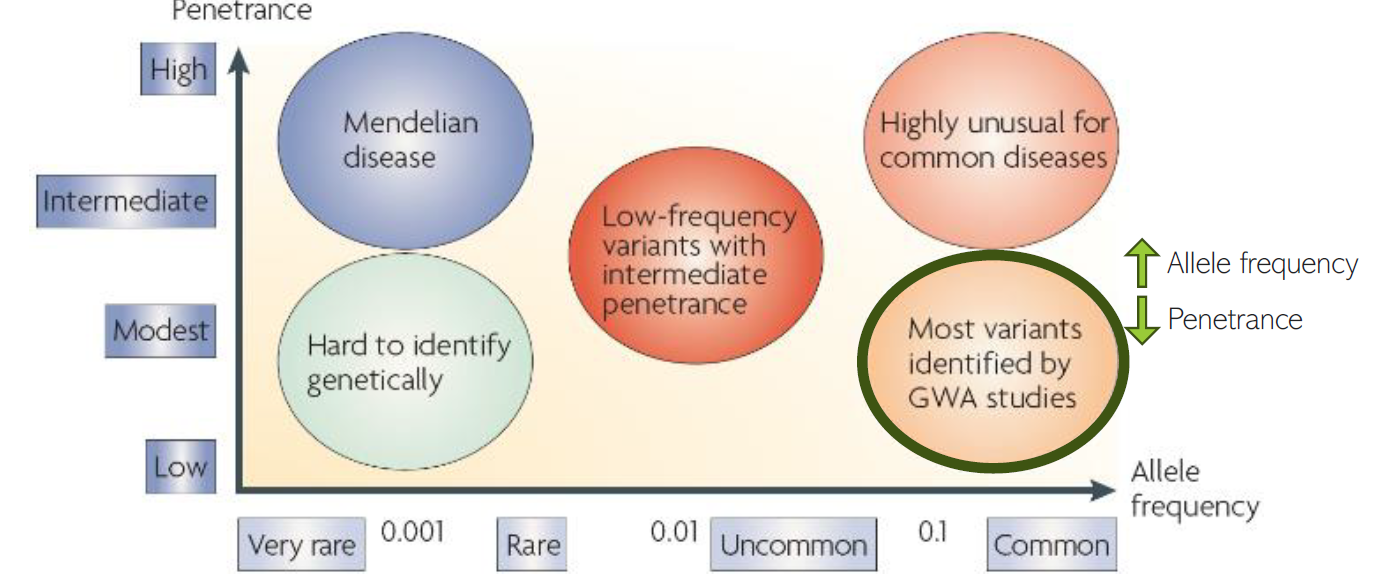
\includegraphics[width = \textwidth]{figs/gwas.png}
\end{figure}

Las variantes estudiadas en GWAS son:
\begin{itemize}
\item Single-Nucleotide Variant (SNV): Cambios de una sola base en el ADN causados por errores durante la meiosis o daño en el ADN de las células germinales.
\item Single-Nucleotide Polymorphism (SNP): SNVs presentes en al menos un 1\% de la población.
\end{itemize}

GWAS analiza grandes cantidades de SNPs (entre 500,000 y 1,000,000 por muestra). Esto es posible gracias a plataformas tecnológicas como Illumina y Affymetrix.

Las herramientas utilizadas en GWAS son:
\begin{itemize}
\item PLINK: Software especializado en la manipulación, resumen y limpieza de datos genéticos.
\item R: Utilizado para análisis estadístico y visualización.
\item Bases de datos:
\begin{itemize}
\item dbSNP: Para obtener información sobre variantes conocidas.
\item GWAS Catalog: Repositorio de estudios GWAS publicados.
\end{itemize}
\end{itemize}

\section{Realizar un GWAS}
El primer paso es \textbf{seleccionar una población de estudio}. Esto depende de la pregunta experimental y hay que tener un tamaño muestral suficiente para asegurar potencia estadística. Si el estudio es dicotómico, habría que tener casos y controles para ver la asociación entre presencia y ausencia. Si por el contrario el estudio es cuantitativo, hay que tener medidas cuantitativas. 

A las personas se las \textbf{genotipa} mediante Whole-genome Sequencing (WGS), whole-exome sequencing (WES) o microarrays (análisis de SNPs concretos para analizar variantes preseleccionadas). 

Una vez secuenciados los datos, hay que \textbf{procesarlos}. En algunos casos hay que anonimizar los datos, ver si hay relaciones familiares entre muestras, sexo, información fenotípica, etc. También es necesario realizar control de calidad. La imputación permite predecir variantes no genotipadas mediante patrones de asociación conocidos. Por último, se realiza un \textbf{test de asociación} para analizar la relación entre variantes genéticas y el fenotipo.

\subsection{Control de calidad}
\subsubsection{Missingness}
En el control de calidad, se mira el missingness o la ausencia tanto por SNP como por individuo. Se eliminan los SNPs o individuos con altos porcentajes de datos ausentes. Los valores recomendados son tener al menos un 95\% de información por muestra y un 95-99\% de información por SNP (call rate).

\begin{figure}[htbp]
\centering
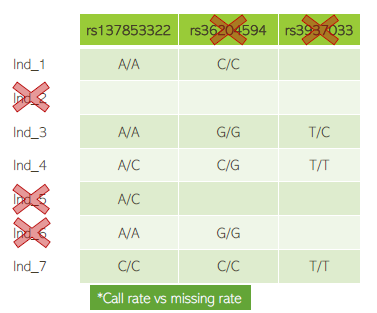
\includegraphics[width = 0.8\textwidth]{figs/missingness.png}
\end{figure}

\subsubsection{Discrepancia por sexo}
Se verifica la concordancia entre el sexo genotípico (tasa de homocigosis en el cromosoma X) y el sexo declarado.

%Para estudiar la discrepancia por sexo, se mira la diferencia entre el sexo asignado y el determinado basado en la información genotípica. Se determina mediante la computación de la tasa de homocigosis de los SNP del cromosoma X.

\subsubsection{Minor Allele Frequency (MAF)}
El Minor Allele Frequency (MAF) se define como la frecuencia del alelo menos frecuente en cada locus. Los GWAS se centran en variantes comunes asociadas a enfermedades en la población. Las variantes raras tienen baja potencia estadística.
Las variantes con un MAF muy bajo también se ven afectadas más fácilmente por errores de genotipado. Se utilizan los siguientes límites: 1-5\% para GWAS de unos cientos o mil individuos y más bajo (0,1\%) para tamaños muestrales más grandes, como UK Biobank.

\subsubsection{Hardy-Weinberg Equilibrium (HWE)}
El equilibrio de Hardy-Weinberg o ley de Hardy-Weinberg establece que en un apareamiento aleatorio tanto las frecuencias alélicas como genotípicas de una población permanecen invariables. Para que este equilibrio se dé, se deben cumplir los siguientes supuestos: apareamiento aleatorio, alelos femeninos y masculinos independientes, frecuencias alélicas idénticas entre machos y hembras, tamaño poblacional grande (infinito), no hay efecto de migración, mutación o selección natural. Para calcular las frecuencias genotípicas, se utiliza la siguiente fórmula:
$$P(G_i) = \sum_{j=1}^6 P(G_i|MT_j) \cdot P(MT_j)$$

\begin{figure}[htbp]
\centering
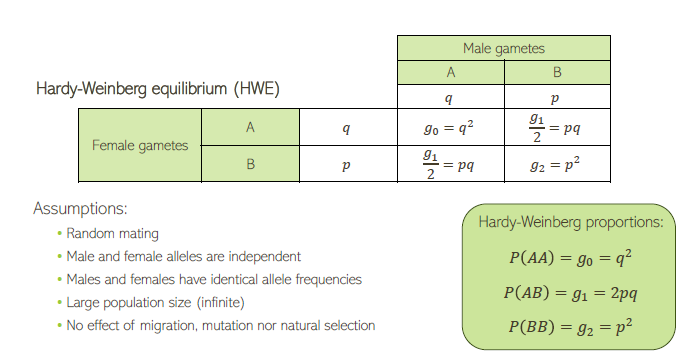
\includegraphics[width = \textwidth]{figs/hwe.png}
\end{figure}

Para asimilar esto, vamos a realizar un ejercicio en el que calculamos el equilibrio Hardy-Weinberg:
\begin{table}[h!]
\centering
\begin{tabular}{|l|c|ccc|}
\hline
\textbf{Mating types} & \textbf{Frequency} & \multicolumn{3}{c|}{\textbf{Frequency of zygotes}} \\ 
\cline{3-5}
                      &                    & \textbf{AA} & \textbf{AB} & \textbf{BB} \\ \hline
MT1: AA x AA          & $g_0g_0 = g_0^2$   & 1           & -           & -           \\
MT2: AA x AB          & $g_0g_1+g_1g_0 = 2g_0g_1$ & 0.5         & 0.5         & -           \\
MT3: AA x BB          & $g_0g_2 + g_2g_0= 2g_0g_2$ & -           & 1           & -           \\
MT4: AB x AB          & $g_1g_1 = g_1^2$   & 0.25        & 0.5         & 0.25        \\
MT5: AB x BB          & $g_1g_2+g_2g_1 = 2g_1g_2$ & -           & 0.5         & 0.5         \\
MT6: BB x BB          & $g_2g_2 = g_2^2$   & -           & -           & 1           \\ \hline
\end{tabular}
\caption{Tabla de frecuencias de tipos de apareamiento y cigotos.}
\label{tab:zygotes}
\end{table}

En base a los resultados de la tabla \ref{tab:zygotes}, las frecuencias genotípicas son:
$$q^2 = P(AA) = 1 \cdot g_0^2 + \frac{2g_0g_1}{2} + \frac{g_1^2}{4} = g_0^2 + g_0g_1 + \frac{g_1^2}{4} = (g_0 + \frac{g_1}{2})^2$$
$$p^2 = P(BB) = \frac{g_1^2}{4} + \frac{2g_1g_2}{2} + g_2^2 = \frac{g_1^2}{4} + g_1g_2 + g_2^2 = (g_2 + \frac{g_1}{2})^2$$
$$2pq = P(AB) = \frac{2g_0g_1}{2} + 1 \cdot 2g_0g_2 + \frac{g_1^2}{2} + \frac{2g_1g_2}{2} = g_0g_1 + 2g_0g_2 + \frac{g_1^2}{2} + g_1g_2 = 2(g_2 + \frac{g_1}{2})(g_0 + \frac{g_1}{2})$$

Para testar las proporciones HWE, se utiliza el test del chi cuadrado.

\begin{figure}[htbp]
\centering
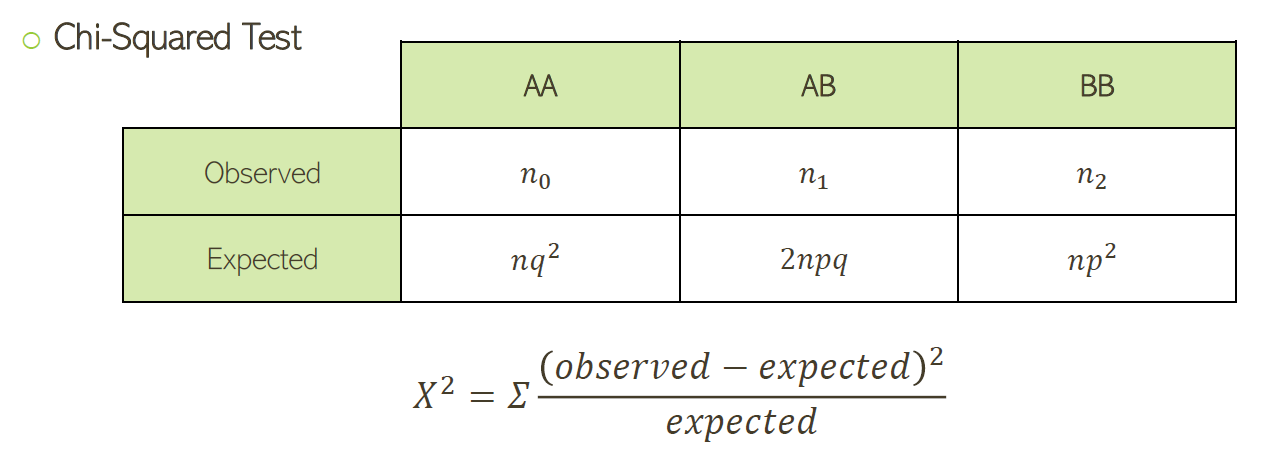
\includegraphics[width = \textwidth]{figs/chi-cuadrado.png}
\end{figure}

Mide lo que difiere los resultados observados con los resultados esperados. El problema es que con los GWAS, este test no es del todo preciso, por lo que se emplea el exact test.

Una vez calculado el HWE y con el test se ve cómo difieren los resultados, se ve si se está violando la ley de HW, es decir, si las frecuencias genotípicas son significativamente diferentes de las esperadas. En GWAS, se asume que desviaciones de HWE se deben a errores del genotipado. En el caso de estudios binarios, el límite del HWE es menos estricto en casos que en controles, ya que la violación de la ley puede indicar una asociación genética real con riesgo a enfermedad. Para estudios cuantitativos, se emplea un p-valor menor a 1e-6. 

\subsubsection{Heterocigosidad}
La heterocigosidad indica la proporción de loci heterocigotos en un individuo, es decir, se refiere a la presencia de los dos alelos en un SNP de un individuo. Se recomienda eliminar todos los individuos que se desvíen $\pm 3 SD$ de la media:
$$HeterozygosityRate_{ind} = \frac{NonMissingCounts - HomozygousGenotypeCount}{NonMissingCounts}$$
Un alto nivel de heterocigosidad se puede deber a una calidad baja de las muestras o contaminación, y unos niveles bajos a inbreeding o una relación entre las muestras.

\subsubsection{Relatedness}
Relatedness es el último paso del control de calidad. En los GWAS más comunes, se asume que no hay asociación entre los participantes del estudio. El grado de relatedness se puede definir como número de alelos compartidos entre los individuos dos a dos. Se mide mediante identity by descent (IBD), que es la proporción de los genomas de dos individuos compartiendo alelos heredados de un ancestro común. 

\begin{figure}[htbp]
\centering
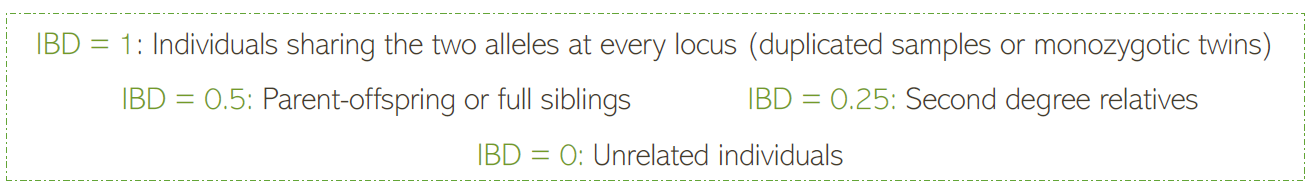
\includegraphics[width = \textwidth]{figs/ibd.png}
\end{figure}

Se diferencian Identity-by-state (IBS) de Identity-by-descent (IBD). En IBS, los alelos compartidos entre individuos son en un locus particular debido a evolución convergente, ancestros comunes o eventos mutacionales similares y se computa como sin información sobre herencia, mientras que en IBD los alelos compartidos entre individuos en un locus particular se debe a un ancestro comun y se debe estimar la probabilidad de heredad la misma copia de un alelo.

En estudios de población estándar, se recomienda eliminar uno de los individuos con un IBD mayor de 0,2. El desequilibrio de ligamiento hace referencia a la herencia conjunta de genes en diferentes loci en el mismo cromosoma en una población concreta. Los SNP están en LD cuando la frecuencia de asociación de sus alelos es superior a la esperada si los loci fueran independientes y estuvieran asociados al azar. 

\section{Práctica: Proyecto HapMap internacional}
El objetivo es elaborar un mapa de haplotipos del genoma humano. La información está disponible gratuitamente en conjuntos de datos públicos. Comenzó con una reunión, celebrada del 27 al 29 de octubre de 2002, y alcanzó su objetivo de completar el mapa en tres años. Se trata de una colaboración entre investigadores de centros académicos, grupos de investigación biomédica sin ánimo de lucro y empresas privadas de Japón, Reino Unido, Canadá, China, Nigeria y Estados Unidos. El HapMap identifica entre 250.000 y 500.000 SNP marcados (casi tanta información cartográfica como los 10 millones de SNP). Cuenta con muestras procedentes de Yoruba, Japón, China y Estados Unidos (residentes en Utah con ascendencia del norte y oeste de Europa).

Los haplotipos son un conjunto de alelos de un cromosomas que se han heredado conjuntamente de un mismo progenitor al estar localizados de forma próxima en el cromosoma. Se puede limitar a un solo gen o a múltiples. Los \textbf{TagSNP} son SNPs representativos en una región del genoma con un alto linkage disequilibrium. 

\begin{figure}[htbp]
\centering
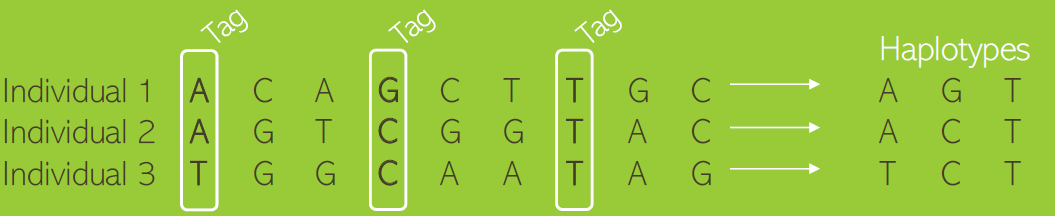
\includegraphics[width = \textwidth]{figs/tagsnp.png}
\end{figure}

El Proyecto Internacional HapMap nació para desarrollar un mapa de haplotipos del genoma humano. 

Durante las prácticas de esta parte de la asignatura, haremos uso de los datos del HapMap para determinar asociaciones entre los SNPs de este estudio y la variable de resultado, en lo que se conoce como estudios de asociación de genoma completo (GWAS).

Como ya hemos visto en clase, el control de calidad es el primer paso en los GWAS. Este proceso es crucial para eliminar las muestras de baja calidad, la contaminación, deshacerse de los errores generados durante el SNP calling o controlar la subestructura de la población, entre otras cosas. Esto es esencial para asegurar que nuestros datos tienen suficiente calidad para realizar las pruebas de asociación.

Como recordatorio, el control de calidad se divide en algunos pasos:
\begin{enumerate}
\item Control for missingness
\item Sex Discrepancy
\item Minor allele frequency
\item Hardy-Weinberg equilibrium
\item Heterozygosity
\item Relatedness
\item Population substructure
\end{enumerate}

En este pipeline, controlaremos los seis primeros pasos. Para ello se utilizará principalmente PLINK, una herramienta que permite estudiar las características de los datos y limpiarlos de forma sencilla y eficaz. También se utilizará R para trazar algunos resultados y ayudar en la determinación de los umbrales (librerías ggplot2 y dplyr).

\subsection{Missingness por individuo y por SNP}
La falta de datos (missingness) se refiere al grado de datos no disponibles a nivel de SNP o de individuo y está directamente asociada con la calidad de los datos. Una buena práctica consiste en eliminar los SNP/individuos con una elevada proporción de omisión.

Para determinar esta proporción, podemos utilizar `--missing` de PLINK. Este flag genera dos archivos que muestran la proporción de SNPs perdidos por individuo y la proporción de individuos perdidos por SNP, respectivamente. 

En este paso, se crean los ficheros plink.lmiss con la información de missigness de los SNP y plink.imiss con la información de missigness de los individuos.

\begin{lstlisting}[language=bash]
plink --bfile HapMap_3_r3_1 --missing --out plink
\end{lstlisting}

Como dice el informe, tenemos 1457897 variantes y 165 personas (80 hombres / 85 mujeres).

\subsection{Estudio de Missingness de SNP}

\begin{lstlisting}[language=R]
snpmiss <- read.table(file="plink.lmiss", header=TRUE)

kable(head(snpmiss), caption = "SNP missingness information") %>%
  kable_styling(bootstrap_options = c("striped", "hover", "condensed", "responsive"), full_width = FALSE) 
\end{lstlisting}

Una vez cargados los datos, los visualizamos:

\begin{lstlisting}[language=R]
p <- ggplot(snpmiss, aes(x=F_MISS)) +
  geom_histogram(color="black", fill="#E69F00", binwidth=.0025) +
  ggtitle('Histogram SNP missingness') +
  ylab('Frequency') +
  geom_vline(xintercept = .02, linetype="dotted",
               color = "black", linewidth=.9)
p 
\end{lstlisting}

\begin{figure}[htbp]
\centering
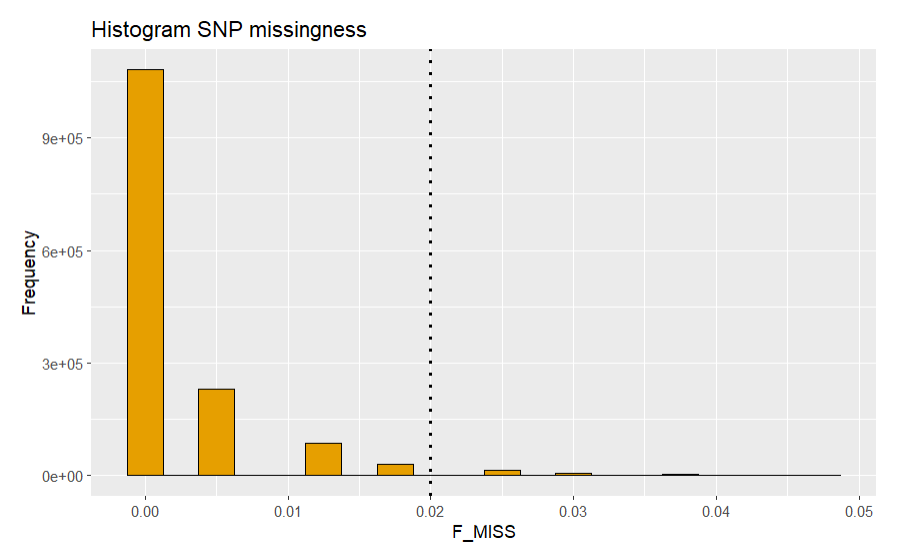
\includegraphics[width = 0.8\textwidth]{figs/hist-snpmiss.png}
\end{figure}

Imaginemos que decidimos fijar un umbral en 0,02. Esto significa que estamos eliminando SNPs con más del 2\% de su información faltante.
\begin{lstlisting}[language=R]
sum(snpmiss$F_MISS > 0.02)
\end{lstlisting}

En total estamos eliminando 27454 valores. Para ver la cantidad de individuos que deben tener una ausencia información para ese SNP para que se elimine, se realiza el siguiente código y el resultado son 4 personas.
\begin{lstlisting}[language=R]
deleted_snp <- snpmiss[snpmiss$F_MISS > 0.02, ]
min(deleted_snp$N_MISS)
\end{lstlisting}

\subsubsection{Estudio de missingness de individuos}
De forma similar a como hemos hecho con el SNP missingness, queremos detectar el missingness individual. Para ello, cargar el archivo que contiene esta información y, representar los individuos falta en un histograma:
\begin{lstlisting}[language=R]
indmiss <- read.table("plink.imiss", header = TRUE)

p <- ggplot(indmiss, aes(F_MISS)) +
  geom_histogram(color="black", fill="#E69F00", binwidth=.0005)

p
\end{lstlisting}

\begin{figure}[htbp]
\centering
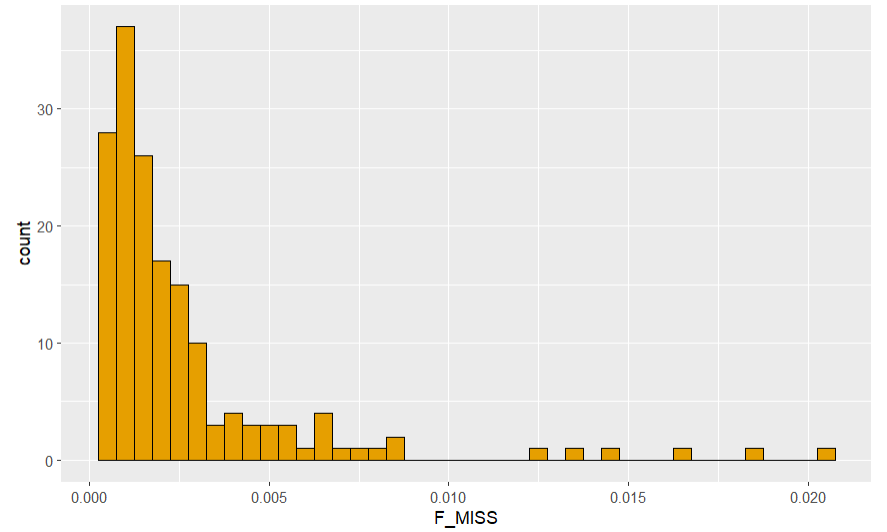
\includegraphics[width = 0.8\textwidth]{figs/hist-indmiss.png}
\end{figure}

Decidimos fijar de nuevo el umbral en 0,02. Esto significa que se eliminan los individuos con más de un 2\% de omisión en sus SNP, que en este caso es una persona.
\begin{lstlisting}[language=R]
sum(indmiss$F_MISS > 0.02)
\end{lstlisting}

Para ver la cantidad de SNPs que deben estar ausentes en un individuo para eliminarlo, se realiza el siguiente cálculo y el resultado son 29584.
\begin{lstlisting}[language=R]
deleted_ind <- indmiss[indmiss$F_MISS > 0.02, ]
min(deleted_ind$N_MISS)
\end{lstlisting}

\subsubsection{Filtrar SNPs e individuos}
Después de representar los resultados, concluimos que el 2\% de missingness es un buen umbral tanto para SNPs como para individuos. Por lo tanto, debemos utilizar `--geno` y `--mind` para eliminar ese porcentaje.

\begin{lstlisting}[language=bash]
# Delete SNPs with missingness >0.02.
plink --bfile HapMap_3_r3_1 --geno 0.02 --make-bed --out HapMap_3_r3_2

# Delete individuals with missingness >0.02.
plink --bfile HapMap_3_r3_2 --mind 0.02 --make-bed --out HapMap_3_r3_3
\end{lstlisting}

Tras analizar el output, vemos que no se ha eliminado ningún individuo. Esto se debe a que, como primero se eliminan los SNP, se recalcula el missingness para los individuos y el que antes sí eliminábamos, ya no cumple con la condición (los SNPs de los que no tenía información son aquellos que se han eliminado por tener poca información de individuos).

%02/12 - Lucía Sánchez
A continuación miramos la discrepancia entre sexos. La discrepancia de sexo se refiere a la diferencia entre el sexo asignado y el determinado. Puede estudiarse con `--check-sex`, que genera un documento con 6 columnas:
\begin{enumerate}
\item FID: family ID
\item IID: individual ID
\item PEDSEX: sex from the pedigree file (1 = male, 2 = female)
\item SNPSEX: sex determined by X chromosome
\item STATUS: problem/ok
\item F: the actual X chromosome inbreeding (homozygosity) estimate. This estimate allows to determine the sex of the individuals, being F < 0.2 assigned to females, and F > 0.8, to males.
\end{enumerate}

Primero utilizamos ese flag para determinar el número de personas con sexo masculino y femenino:
\begin{lstlisting}[language=bash]
plink --bfile HapMap_3_r3_3 --check-sex --out plink
\end{lstlisting}

Ese fichero se carga en R y se genera un histograma con F estimado:
\begin{lstlisting}[language=R]
sex <- read.table("plink.sexcheck", header = TRUE)
p <- ggplot(sex, aes(F)) +
  geom_histogram(color="black", fill="#E69F00", binwidth=.005)
p
\end{lstlisting}

Para ver el número de hombres y mujeres predichos:
\begin{lstlisting}[language=R]
#males
sum(sex$SNPSEX == 1)

#females
sum(sex$SNPSEX == 2)
\end{lstlisting}
Obtenemos 81 hombres y 84 mujeres. Ahora queremos ver si hay alguna discordancia entre el sexo predicho y el computado:
\begin{lstlisting}[language=R]
discordance <- sex[sex$PEDSEX != sex$SNPSEX,]
discordance
\end{lstlisting}

Vemos que hay un individuo que discrepa, por lo que queremos filtrarlo. Generamos un fichero .txt con el FID e IID de la persona problemática.
\begin{lstlisting}[language=bash]
grep "PROBLEM" plink.sexcheck | awk '{print $1, $2}' > sex_discrepancy.txt
\end{lstlisting}

Posteriormente utilizamos el flag --remove para eliminar los individuos en el fichero txt.
\begin{lstlisting}[language=bash]
plink --bfile HapMap_3_r3_3 --remove sex_discrepancy.txt --make-bed --out HapMap_3_r3_4
\end{lstlisting}

Ahora analizamos minor allele frequency (MAF). El MAF se refiere a la frecuencia del alelo menos frecuente en un locus. Debemos eliminar los SNP con un MAF bajo porque la potencia estadística de los GWAS no permite detectar asociaciones si la frecuencia del alelo es demasiado baja. Generamos un fichero .txt con los SNPs autosomales y después eliminamos aquellos con el MAF más pequeño. 
\begin{lstlisting}[language=bash]
# Select autosomal SNPs (from chromosomes 1 to 22).
awk '{ if ($1 >= 1 && $1 < 23) print $2}' HapMap_3_r3_4.bim > snp_1_22.txt
#Remove unlisted variants
plink --bfile HapMap_3_r3_4 --extract snp_1_22.txt --make-bed --out HapMap_3_r3_5
\end{lstlisting}

A continuación utilizamos el flag --freq para computar el MAF en los cromosomas autosomales.
\begin{lstlisting}[language=bash]
plink --bfile HapMap_3_r3_5 --freq --out plink
\end{lstlisting}

Cargamos el fichero generado y representamos la distribución de MAF en un histograma, estableciendo un límite del 5\%.
\begin{lstlisting}[language=R]
maf_freq <- read.table("plink.frq", header = TRUE)
p <- ggplot(maf_freq, aes(MAF)) +
	geom_histogram(color="black", fill="#E69F00", binwidth=.005) +
	geom_vline(xintercept = .05, linetype="dotted", color = "black", linewidth=.9)
p
\end{lstlisting}

Estamos eliminando 1073226 SNPs y quedándonos con 325318.
\begin{lstlisting}[language=R]
#deleting
sum(maf_freq$MAF >= 0.05)
#retaining
sum(maf_freq$MAF < 0.05)
\end{lstlisting}

Eliminamos los SNPs.
\begin{lstlisting}[language=bash]
plink --bfile HapMap_3_r3_5 --maf 0.05 --make-bed --out HapMap_3_r3_6
\end{lstlisting}

El siguiente paso es eliminar los SNPs que no estén en equilibrio Hardy-Weinberg. El equilibrio de Hardy-Weinberg (HWE) establece que, en un apareamiento aleatorio, las frecuencias alélicas y genotípicas permanecen constantes o estables en una población si no se introducen factores perturbadores. `--hardy` escribe una lista de recuentos de genotipos y estadísticas de la prueba exacta de equilibrio Hardy-Weinberg.
\begin{lstlisting}[language=bash]
plink --bfile HapMap_3_r3_6 --hardy --out plink
\end{lstlisting}

Posteriormente elegimos los SNPs con un p-valor HWE < 0,0001.
\begin{lstlisting}[language=bash]
awk '{ if ($9 <0.00001) print $0 }' plink.hwe > plinkzoomhwe.hwe
\end{lstlisting}

Y ahora creamos los histogramas:
\begin{lstlisting}[language=R]
hwe <- read.table("plink.hwe", header = TRUE)
hwe
p <- ggplot(hwe, aes(P)) +
  geom_histogram(color="black", fill="#E69F00", binwidth=.05)
p

hwe_zoom <- read.table("plinkzoomhwe.hwe", header = FALSE)
hwe_zoom
p <- ggplot(hwe_zoom, aes(V9)) +
  geom_histogram(color="black", fill="#E69F00")
p
\end{lstlisting}

\section{Consideraciones de GWAS}
En cuanto al diseño del estudio, pueden diferenciarse los estudios basados en población, en familia o en poblaciones aisladas.

\subsection{Population-based GWAS}
Se trata de un estudio de asociación genética con individuos no emparentados. El estudio más común es uno de casos y controles, siendo los casos personas con presencia de un fenotipo y los controles ausencia del mismo. Los individuos pueden seleccionarse activamente y los controles se pueden emparejar con los casos (con respecto al sexo, factores de riesgo, ...). Se realiza un reclutamiento activo. Estos estudios tienen buena potencia y son rentables si la frecuencia de la enfermedad en la población es baja (<20\%). Si la frecuencia de los casos es mayor que la frecuencia basada en población, se debe ajustar por covariantes durante el análisis estadístico. Los casos y controles que no se genotipen conjuntamente deben tener una corrección (batch correction) para ajustar por covariables.

Los estudios de casos y controles se pueden clasificar en estudios retrospectivos y prospectivos. En los \textbf{estudios retrospectivos}, los sujetos se seleccionan en función de su estado de enfermedad. Se suele utilizar con enfermedades raras, ya que no es viable escoger participantes y esperar a que generen la enfermedad. Se obtienen los datos genéticos y ambientales.

En los \textbf{estudios prospectivos}, se establece una cohorte y se realiza un genotipado base de todos los sujetos. Se realiza un seguimiento de los individuos y se observa si hay un desarrollo de la enfermedad. Aquellos que la desarrollen pasan a ser casos, y aquellos que no serán los controles. 

Las ventajas es que estos estudios son muy rentable para asociaciones a gran escala, pero tiene la desventaja de obtener subgrupos poblacionales, generando asociaciones falsas debido a las subpoblaciones.

\subsection{Family-based GWAS}
Este estudio utiliza sujetos recogidos en familias, y se utilizó frecuentemente en los inicios de GWAS. En el caso del trío caso-padres, se genotipa a la descendencia afectada y a los padres. Se compara entre el número de alelos marcadores transmitidos de padres a descendientes con el número de alelos no transmitidos. Se puede tralizar la prueba de desequilibrio de transmisión (TDT) o prueba de asociación para identificar el vínculo genético entre un marcador genético (SNP) y un rasgo (fenotipo). Examina la segregación de un alelo dentro de una familia. La ventaja es que es robusto frente a estratificación poblacional y con enfermedades de baja prevalencia (< 1\%). Además, se estudian los efectos de un alelo en un fenotipo individual de sus efectos indirectos en miembros familiares cercanos. No obstante, se requiere un tamaño muestral más grande que el GWAS poblacional para alcanzar la misma potencia estadística y es menos eficiente en el caso de enfermedades de aparición tardía.

\subsection{Poblaciones aisladas}
Las poblaciones aisladas son grupos separado de sus poblaciones vecinas por barreras (geográficas, culturales o lingüísticas) y que tienen un flujo genético mínimo desde ellas. Estas poblaciones aisladas han permanecido aisladas durante un periodo prolongado, teniendo un flujo genético restringido con las poblaciones vecinas. Estos estudios tienen una mayor precisión de imputación que otras pruebas con un desequilibrio de ligamiento de largo alcance. 
Los descubrimientos en poblaciones aisladas son muy difíciles de replicar en otras poblaciones. Así, variantes funcionales raras pueden estar presente en mayor frecuencia en poblaciones aisladas, habiendo así una potencia aumentada para estudios de asociación de estas variantes.

\subsection{Subestructura poblacional - práctica}
En esta práctica estudiaremos relatedness y la estratificación poblacional. La estratificación poblacional puede ser la principal fuente de confusión. Ejemplo: estudio de casos y controles, en el que las diferencias genotípicas entre casos y controles se deben a los distintos orígenes de la población (casos: europeos, controles: asiáticos) y no a un efecto sobre el riesgo de enfermedad. La confusión se debe a que la subestructura de la población no está distribuida por igual entre los grupos de casos y controles. Así, una señal de asociación surgirá no por una asociación entre un fenotipo y un SNP, sino por diferencias de frecuencia alélica entre las poblaciones que comprenden los casos y los controles. Esto tiene dos soluciones: eliminar los individuos de ascendencia divergente o establecer la ascendencia como covariable/efecto aleatorio en modelos mixtos.

Los métodos para identificación de individuos con diferencias a larga escala en ascendencia es mediante una PCA (principal component analysis) o MDS (multidimensional scaling). MDS calcula la proporción de alelos compartidos entre cada par de individuos para identificar la variación genética para cada individuo. Los resultados se muestran en un gráfico para explorar la distribución de individuos en los datos. Por ejemplo, estudio genético que incluya sujetos de Asia y Europa. El análisis MDS revelaría que los asiáticos son genéticamente más parecidos entre sí que a los europeos.

%04/12 - Lucía Sánchez
\chapter{Análisis estadístico o de asociación}
La imputación permite predecir otros SNPs no secuenciados debido a que se heredan conjuntamente, ampliando así la información de los SNPs. Los softwares que se pueden utilizar son:
\begin{itemize}
\item \textbf{IMPUTE2 y MACH}: utilizan un modelo de Markov oculto (HMM) para estimar los genotipos que faltan, mediante la inferencia de haplotipos y el uso de parámetros genéticos previamente especificados, como las tasas de mutación y de recombinación
\item \textbf{BEAGLE}: no necesita tales parámetros. Estima los valores que faltan mediante el uso de haplotipos agrupados localmente con algoritmos HMM y de maximización de expectativas (EM).
\end{itemize}

El test de asociación se realiza después de la imputación. El test de asociación que se realice depende del fenotipo (binario o continuo), el control de covariantes (edad, sexo) y la estructura poblacional (estratificación u homogeneidad), pudiendo ser regresiones lineales, regresiones lineales múltiples, modelos lineares mixtos, regresiones logísticas, etc. Los tipos de análisis que se pueden encontrar en función de la dominancia son:
\begin{itemize}
\item \textbf{Modelo dominante:} La presencia del alelo B aumenta el riesgo de enfermedad en la misma medida para los genotipos BB y AB, en comparación con el riesgo de referencia para los AA.
\item \textbf{Modelo codominante o aditivo:} Cada copia adicional del alelo B aumenta el riesgo de enfermedad de forma aditiva, o por el contrario, aumenta el efecto protector.
\item \textbf{Modelo recesivo:} Se necesitan dos copias del alelo B para expresar la característica fenotípica relacionada con este alelo.
\end{itemize}

\section{Tipos de test de asociación}
\subsection{Modelos lineares}
Se describen mediante la fórmula:
$$y = \beta_0 + \beta_1 \cdot X_{1i} + \epsilon_1$$

Siendo $y$ la variable dependiente (respuesta/outcome), $\beta_0$ el término constante del modelo, $\beta_1$ el coeficiente de regresión, $X_{1i}$ la variable independiente o predictora y $\epsilon_1$ el término del error. $i$ representa el número de observaciones o muestras.

Los cambios que se producen en el outcome (y) se puede modelar como una función lineal de la variable independiente. Así, un cambio en la variable independiente produce un cambio en la variable dependiente, siendo ésta numérica. 

Un ejemplo: Se desea estimar si el tabaco (medido como el número de cigarrillos fumados al mes) influye en el volumen residual pulmonar (VR: volumen de aire que queda en los pulmones tras una espiración máxima). Si existe una asociación entre el tabaco y el VR, el número de cigarrillos (variable independiente) se asociaría con una reducción del VR (variable dependiente)

En este caso, la variable predictora va a ser categórica, representando los distintos SNPs. Normalmente, el estimador (la pendiente) suele estar relacionado con el p-valor. 

\subsection{Modelos de regresión lineal múltiple}
Se incluyen otros predictores o covariables. Los términos en la variable dependiente se modelan con todos los predictores independientes. Una manera de regular la estratificación de la población es metiéndolo como covariable.

Siguiendo con el ejemplo previo, nos damos cuenta de que el volumen residual puede verse afectado no sólo por el número de cigarrillos fumados al mes, sino también por la edad y el sexo. Ahora tendremos tres variables independientes para probar la dependiente: tabaco, sexo y edad.

\subsection{Modelos lineares mixtos}
Estos modelos sirven para modelar estructuras de datos más complejas. Las variables predictoras se dividen en dos:
\begin{itemize}
\item \textbf{Efecto fijo:} son las variable que se espera que tengan un efecto en la variable respuesta. Un ejemplo sería los SNP y el entorno o las covariables clínicas.
\item \textbf{Efectos aleatorios:} no nos interesa su impacto en la variable de respuesta, pero sabemos que pueden estar influyendo en los patrones que observamos, por lo que queremos separarlos del modelo para ver cómo verdaderamente el efecto fijo afecta al outcome. Aquí se contarían variables categóricas que queremos controlar.
\end{itemize}

Un ejemplo sería un estudio de la deprivación del sueño. Se restringe el tiempo de sueño de 18 individuos y la reacción de su organismo durante 10 días. El objetivo es determinar cómo cambia la reacción de los individuso durante su deprivación de sueño. Si se mide como regresión lineal simple, la variabilidad va cambiando. Si se clusteriza cada dato por individuo, se puede ver que la recta que se traza es más ajustada a los datos, demostrando que hay una estructura compleja que no se puede determinar por un modelo lineal.

\begin{table}[htbp]
\centering
\begin{tabular}{p{7cm}|p{7cm}}
Modelo de regresión lineal & Modelos mixtos \\ \hline
Suponen una relación lineal entre las variables dependientes e independientes. & Relajan el supuesto de independencia entre las observaciones. \\
\\
Adecuado para analizar datos con una estructura simple (se supone que las observaciones son independientes entre sí). & Adecuado para analizar datos con una estructura agrupada (las observaciones están anidadas dentro de grupos / mediciones repetidas en los mismos sujetos). \\
\\
Los modelos de regresión lineal suelen incluir efectos fijos: parámetros asociados a las variables predictoras. Estos efectos son constantes en todos los niveles de cualquier variable de agrupación. & Los modelos mixtos incluyen efectos fijos (como los modelos lineales) y efectos aleatorios (captan la variabilidad a distintos niveles).\\
\\
Tareas de regresión simple: se desea predecir una variable de resultado continua a partir de una o más variables predictoras. & Se utilizan en análisis de datos longitudinales, análisis de medidas repetidas y modelización jerárquica. Son apropiados cuando los datos no son independientes y se desea tener en cuenta las correlaciones dentro del grupo o la variabilidad específica de los sujetos.
\end{tabular}
\end{table}

\subsection{Regresión logística}
La regresión logística sigue la fórmula:
$$y = \frac{e^{(\beta_0 + \beta_1X_{1i)}}}{1 + e^{(\beta_0 + \beta_1X{1i})}}$$

Los cambios en la variable dependiente (y) pueden modelizarse como una función logística de las variables independientes. Hay dos variantes:
El modelo de regresión logística múltiple es como la lineal múltiple, pero logística, es decir, se añaden varias variables independientes. El modelo multinomial cuenta con una variable dependiente con más de dos categorías.

Siguiendo con el ejemplo, nos interesa detectar si existe una asociación entre el número de cigarrillos: (variable independiente continua) y el volumen residual inferior a 1 litro (variable dependiente binaria: sí/no). En la regresión logística múltiple, se añadiría sexo como covariable, mientras que en la regresión logística multinomial la variable dependiente tendría más de dos categorías.

\section{Visualización de datos}
El plot se denomina como Manhattan plot. Las asociaciones significativas se muestran en la parte superior del gráfico. El eje x va por orden en los distintos cromosomas. 

\begin{figure}[htbp]
\centering
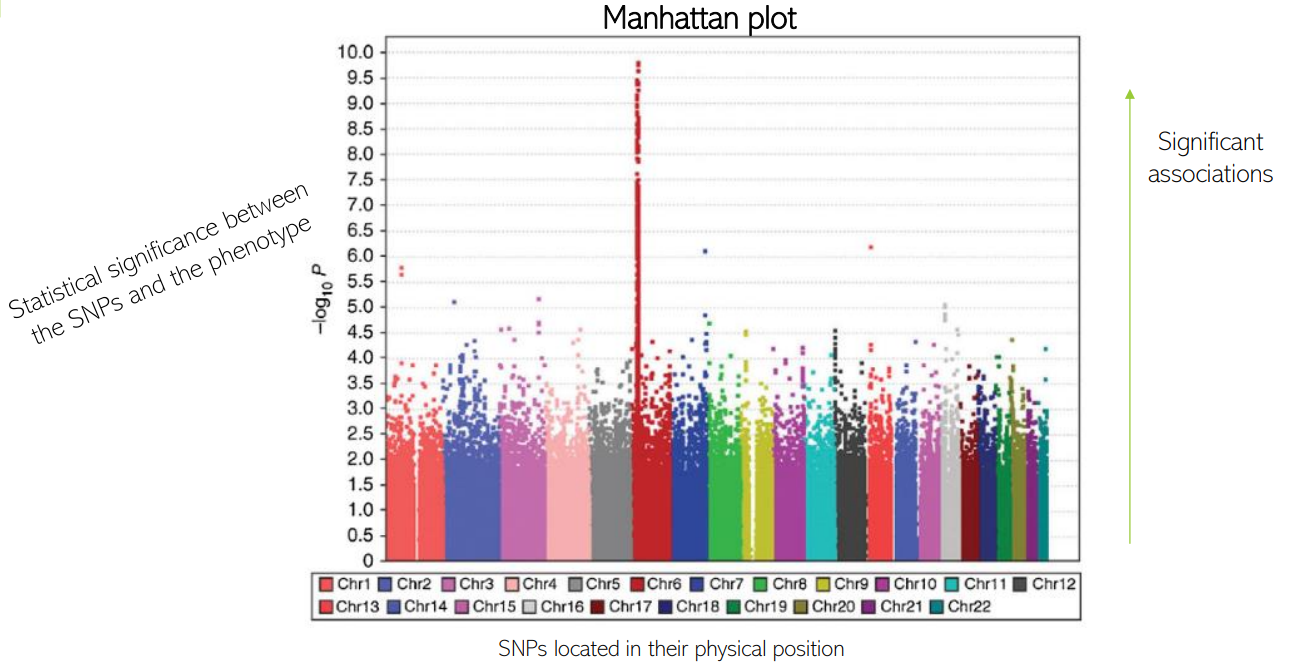
\includegraphics[width = \textwidth]{figs/manhattan-plot.png}
\end{figure}

\section{Nivel de significancia de GWAS}
A la hora de mirar el nivel de significancia de GWAS, nos encontramos con el problema del testeo múltiple. El p-valor representa la probabilidad de obtener resultados tan extremos como los observados si la hipótesis nula es correcta. La hipótesis nula dice que no hay una relación significativa entre el predictor y la variable respuesta. El nivel de significancia se suele poner en 0,05. 

Por ejemplo, estamos probando (hipótesis nula) que no hay una relación significativa entre el predictor (SNP, edad y sexo) con la variable respuesta (volumen residual). Si el p-valor es 0,03, si no hubiera una relación entre esas variables (y la hipótesis nula fuera cierta), la probabilidad de tener resultados tan extremos como los observados sería de 0,03. 

Con un nivel de significancia de 0,05, todavía hay una probabilidad de que no haya una relación significativa, aunque sea pequeña. Esto no es un problema cuando se realiza un solo análisis, pero cuando se realizan muchos, se incrementa el número de falsos positivos. Por ello, se debe controlar el testo múltiple y ajustar el p-valor. Esto se puede realizar de varias formas:
\begin{itemize}
\item \textbf{Corrección de Bonferroni:} divide el nivel de significancia por el número de análisis realizados para ver el nivel de significancia que se debe comprobar en cada análisis individual. No obstante, es algo restrictivo, incrementando los falsos negativos.
\item \textbf{False Discovery Rate (FDR):} se describió por Benjamini y Hochberg en 1995, y monitoriza el número de falsos positivos en relación al número de resultados positivos, siendo así menos estricto.
\end{itemize}

%09/12 - Fátima
\chapter{Epidemiología molecular: introducción a la inferencia causal}
Los biobancos son grandes estudios poblacionales que siguen a personas aparentemente sanas. En el portal de \href{https://portal.gdc.cancer.gov/analysis_page?app=}{TGCA} se han creado algunas herramientas que permiten construir una cohorte: obtener los pacientes con un tipo de cáncer para sacar cierta información. Se pueden ver los tipos de datos disponibles y aplicando distintos filtros. Como bioinformáticos, no nos gusta acceder a las bases de datos mediante front-end, ya que esto solo sirve para consultas pequeñas. Nosotros accederemos desde R (script en la carpeta de prácticas, \texttt{tcga.R}).

Para prácticamente todos los biobancos existen APIs para acceder y un paquete de R para poder minar las bases de datos. En este caso, como queremos acceder a TGCA, utilizaremos el paquete de TCGAretriever.

 \section{Correlación vs causalidad}
 La correlación no implica causalidad. Hay muchos ejemplos en los que hay variables confusoras que hacen que haya correlación entre ambos eventos, pero no causalidad: ventas de helados y ataques de tiburones (verano como variable confusora), consumo de chocolate y premios Nobel en un país (país con gran inversión y poder adquisitivo). 
 
Hay veces que es complicado ver si algo es causal o no. La ciencia ha tratado de investigar la causalidad en variables asociadas en modelos animales y ensayos clínicos. En ratones, se puede simular la situación mediante knock-outs para demostrar causalidad de forma directa, pero la experimentación con animales es complicada y de aquí a unos años puede estar incluso prohibida. En el caso de los ensayos clínicos, se pueden buscar individuos con características que se quieren simular, se puede ver el outcome. No obstante, son muy caros y muy largos. Otra opción es mediante modelos digitales que permitan simular \textit{in silico} la asociación y causalidad con distintos fenotipos. Ahora que hay tantos biobancos y se invierte tanto dinero en ellos, se pueden obtener muchos datos observacionales. 

\section{Inferencia causal}
La inferencia causal nos permite sacar conclusiones causales a partir de los datos observacionales de los que a priori solo podemos sacar asociaciones. Para ver causalidad habría que comparar a un mismo individuo en dos situaciones, pero es complicado obtener esos estados (no puedes comparar el efecto de una aspirina en una persona comparando su estado tomándosela y no tomándosela, ya que no se puede realizar ambas). 

El efecto causal de un tratamiento en un mismo individuo es la diferencia entre el valor del outcome si el individuo se trata y el valor del outcome si no se trata. No obstante, es imposible obtener esos dos outcomes. 

Se hizo un estudio en el que se miró si el consumo de alcohol tiene relación con sufrir un infarto. Idealmente, se buscaba tener datos de las distintas personas sin consumo de alcohol y con consumo, midiendo el tiempo hasta que sufre un infarto. Cada una de las dos columnas tiene una distribución (función de probabilidad). Con esta información, lo que tenemos en un estudio observacional es para una persona, una variable que dice si toma o no alcohol y el tiempo de supervivencia en su grupo correspondiente. Esto es un problema de valores perdidos: sabiendo la distribución de los datos (de estudios observacionales anteriores), podemos simular y rellenar la tabla con los valores faltantes (el tiempo hasta sufrir un infarto para cada persona en el grupo faltante).

\subsection{Neyman-Rubin Causal Model}
El teorema de Rubin dice que si la variable es totalmente independiente del outcome que se mide (si tomar alcohol y tener un infarto es independiente), no se necesita para cada persona los dos valores, ya que se puede sustraer la media de las dos variables y se obtiene una estimación muy buena que correspondería a tener para cada individuo los dos valores y extraer la media. Hay variantes genéticas que predisponen al consumo de alcohol, y variantes genéticas que predisponen al infarto. Si las variantes son diferentes, se puede clasificar a cada persona en su grupo.

\section{Genes como variables instrumentales}
De forma aleatoria, nosotros tenemos un genotipo u otro, por lo que se puede considerar como variable instrumental. Esto sirve para la \textbf{mendelian randomization}, la cual se basa en el supuesto de que las variantes genéticas aportan una fuente de variación exógena en la exposición.

Hay muchos supuestos:
\begin{enumerate}
\item La variante genética tiene que estar asociada con el trait asociado
\item La variante genética no puede estar asociada con ninguna variable confusora
\item La variante genética no puede estar asociada directamente con el outcome
\end{enumerate}

Esto se puede realizar en R con el paquete \texttt{MendelianRandomization}.

betaX y betaXse son vectores numéricos que describen las asociaciones de las variantes genéticas con la exposición. 
betaX son los coeficientes beta de los análisis de regresión univariable de la exposición/tratamiento sobre cada variante genética. 
betaXse son los errores estándar.
betaY y betaYse son vectores numéricos que describen las asociaciones de las variantes genéticas con el resultado: 
betaY son los coeficientes beta de los análisis de regresión del resultado en cada variante genética 
betaYse son los errores estándar
Correlación es una matriz con las correlaciones con signo entre las variantes. Si no se proporciona una matriz de correlación, se asume que las variantes no están correlacionadas.
exposition es una cadena de caracteres que indica el nombre del factor de riesgo, por ejemplo, LDL-colesterol
outcome es una cadena de caracteres que indica el nombre del resultado, por ejemplo, cardiopatía coronaria. 
snps es un vector de caracteres que contiene los nombres de las distintas variantes genéticas (SNP) del conjunto de datos, por ejemplo rs12785878. 

No es necesario nombrar la exposición, el resultado o los SNPs, pero estos nombres se utilizan en las funciones gráficas y pueden ser útiles para realizar un seguimiento de los distintos análisis.

%11/12 - Jorge de la Barrera jdelabarrera@cnic.es
\chapter{Genetic Susceptibility (Polygenic Risk Scores)}
\section{La búsqueda de variantes causantes de enfermedad}
Las enfermedades monogénicas tienen pocas variantes, pero con mucho efecto. Las enfermedades poligénicas van al revés, teniendo muchas variantes pero con poco efecto. Entre medias están las enfermedades oligogénicas. 

\begin{figure}[htbp]
\centering
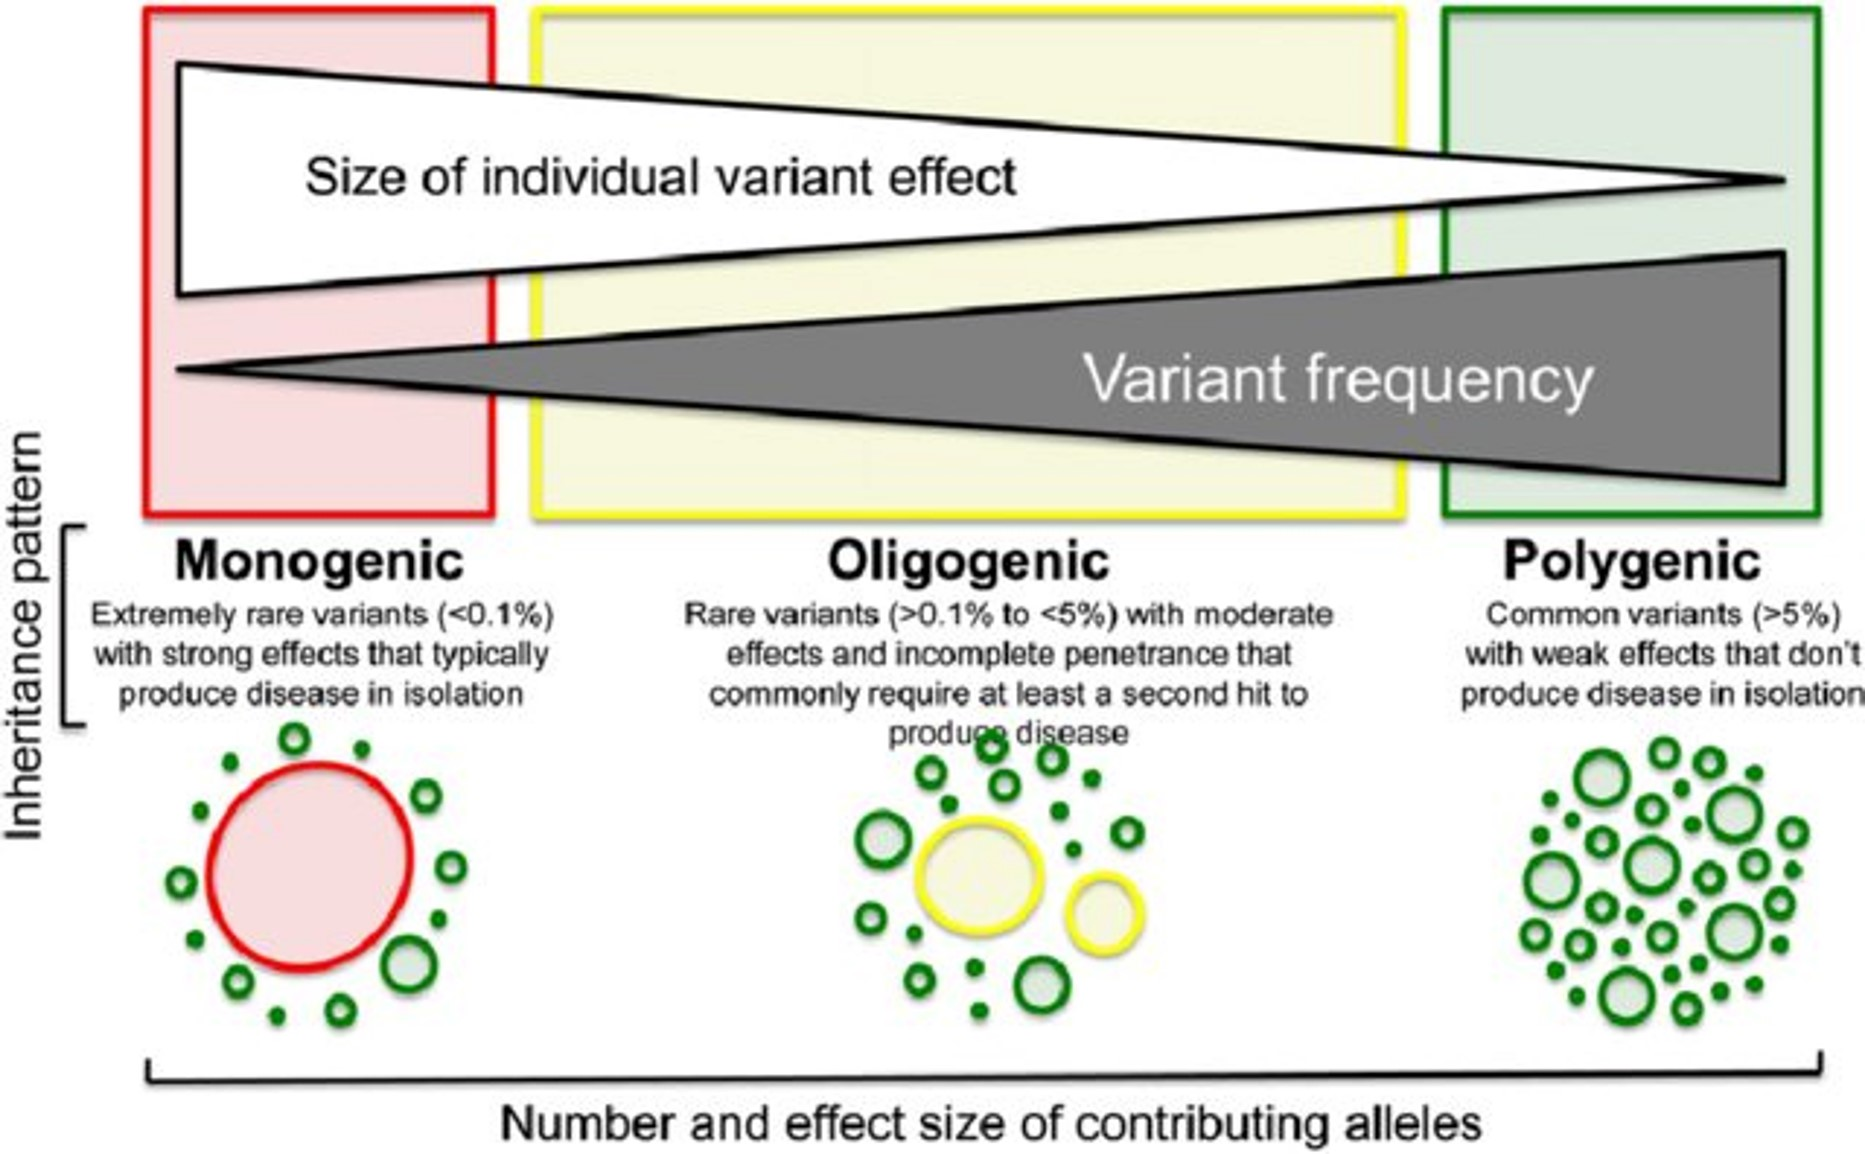
\includegraphics[width = 0.8 \textwidth]{figs/Imagen1.jpg}
\end{figure}

Los trastornos monogénicos están causados por una única variante de alta penetrancia en un gen. 
Son poco frecuentes en la población y se asocian a un alto riesgo relativo de desarrollar la enfermedad. 
Por ejemplo, la enfermedad de Huntington es un trastorno monogénico.

Los trastornos poligenéticos están influidos por los efectos combinados de múltiples SNP comunes, cada uno con un pequeño efecto sobre el riesgo de enfermedad. 
Por ejemplo, la diabetes tipo 2 es un trastorno poligénico.

\section{Polygenic Risk Score (PRS)}
El PRS (polygenic risk score) es un número que estima la predisposición genética de un individuo a una enfermedad o rasgo específico. Proporciona una medida de la predisposición genética. Esta estimación se basa en su perfil genotípico y en datos estadísticamente ponderados de GWAS relevantes. Se calculan combinando información de miles de variantes genéticas, cada una con tamaños de efecto pequeños.

\begin{figure}[htbp]
\centering
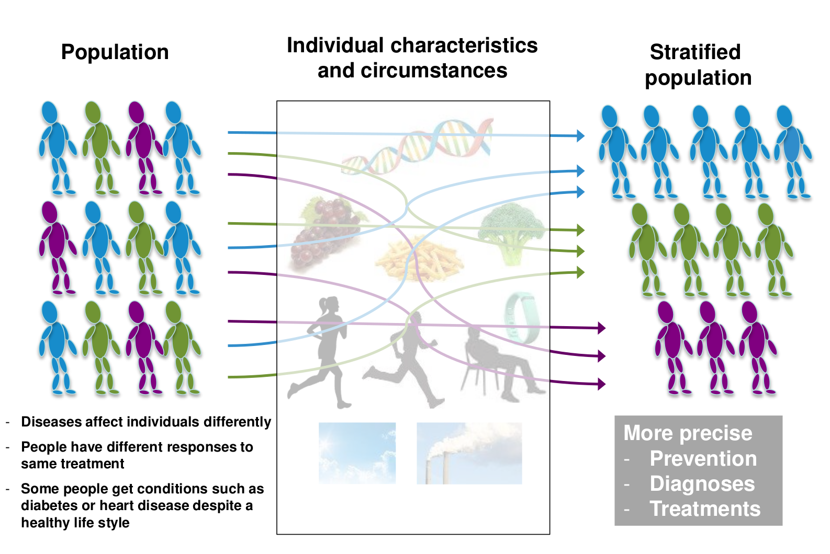
\includegraphics[width = 0.8 \textwidth]{figs/Imagen2.png}
\end{figure}

Las enfermedades monogénicas suelen ser raras, pero las poligénicas comunes. Si nosotros somos capaces de tener en un score el riesgo, se pueden estratificar los individuos según su riesgo, creando predicciones más ajustadas y políticas de prevención más acorde. Así, los PRS permiten realizar una prevención más precisa, mejorar el diagnóstico, y mejorar los tratamientos. En resumen:
\begin{itemize}
\item \textbf{Prevención selectiva:}
Estratificar a los individuos según su riesgo genético de desarrollar diversas enfermedades comunes.
Optimizar el uso del cribado y los tratamientos preventivos.
Informar a los programas de cribado de la población identificando a los individuos con mayor riesgo.

\item \textbf{Diagnóstico temprano:}
Facilitar el diagnóstico de enfermedades complejas, especialmente en conjunción con otros factores clínicos.
Afinar las estimaciones de riesgo en familias con antecedentes de determinadas enfermedades, especialmente cuando se combinan con pruebas de riesgo monogénico.

\item \textbf{Intervenciones personalizadas:}
Mejorar la atención personalizada a los pacientes.
Orientar las decisiones terapéuticas al proporcionar información sobre la probabilidad de que un individuo responda a terapias específicas.
Informar sobre el pronóstico al ofrecer información sobre la posible evolución de la enfermedad y sus resultados.
\end{itemize}

\begin{figure}[htbp]
\centering
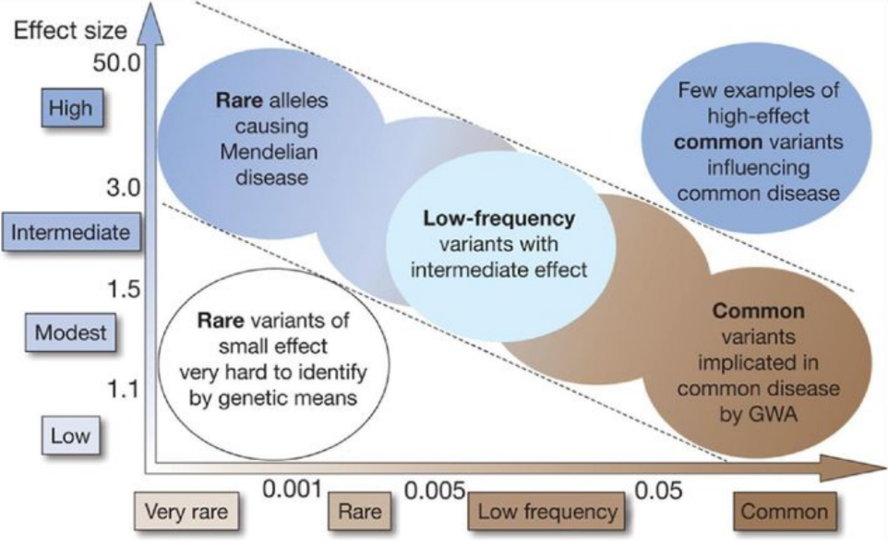
\includegraphics[width = 0.8 \textwidth]{figs/Imagen3.png}
\end{figure}

\subsection{Entendiendo los PRSs}
Las PRS son puntuaciones genéticas que \textbf{combinan los efectos} de muchas variantes genéticas (SNPs) para evaluar la \textbf{predisposición de un individuo} a un rasgo o enfermedad específica.

Las PRS se desarrollan \textbf{utilizando datos de estudios de asociación de genoma completo (GWAS)} . 	Estos estudios identifican los SNP asociados a un rasgo o enfermedad concretos mediante el análisis de los genomas de grandes poblaciones. Su fórmula general es:
$$PRS = \sum (efecto del SNP \cdot alelo portado)$$.

Esta fórmula calcula la PRS sumando el número de alelos de riesgo que porta una persona en cada SNP relevante, ponderado por el tamaño del efecto de cada alelo.

Entre los usos del PRS se encuentran:
\begin{itemize}
\item \textbf{Predicción de riesgos genéticos}: Las PRS pueden estimar el riesgo genético de un individuo a lo largo de su vida de desarrollar determinadas enfermedades, como cardiopatías, diabetes o cáncer.
\item \textbf{Complementación de factores clínicos y ambientales}: Las PRS pueden utilizarse con otros factores de riesgo, como los antecedentes familiares, el estilo de vida y los indicadores clínicos, para ofrecer una imagen más completa del riesgo global de una persona.
\item \textbf{Mejorar el diagnóstico y el tratamiento personalizado}: Las PRS pueden ayudar a afinar el diagnóstico, sobre todo en el caso de enfermedades con síntomas que se solapan. También pueden orientar las decisiones de tratamiento, ya que las personas con diferentes PRS pueden responder de forma diferente a los mismos medicamentos.
\end{itemize}

Consideraciones importantes:
\begin{itemize}
\item Los PRS son estimaciones de riesgo, no diagnósticos. Indican una predisposición, no la certeza de desarrollar una enfermedad.
\item Las PRSs actuales suelen explicar sólo una pequeña fracción de la variación de un rasgo o enfermedad. Esto se debe a que los factores ambientales y las interacciones gen-ambiente también desempeñan un papel importante.
\item La precisión de las PRSs depende de factores como el tamaño y la diversidad de los GWAS utilizados para desarrollarlas.
\item La mayoría de las PRSs se han desarrollado utilizando datos de individuos de ascendencia europea, lo que limita su precisión y aplicabilidad a otras poblaciones.
\item Las PRSs evolucionan rápidamente a medida que avanza la investigación y se dispone de más datos.
\end{itemize}

\subsection{Fundamentos teóricos del PRS}
El PRS se basa en dos fundamentos. El primero es el \textbf{principio de la herencia poligénica}.
La herencia poligénica se refiere al concepto de que múltiples genes contribuyen a un rasgo o enfermedad.
El segundo es la \textbf{heredabilidad y su relación con la PRS}.
La heredabilidad es la proporción de variación fenotípica en una población que puede atribuirse a factores genéticos. La heredabilidad SNP se refiere a la proporción de varianza fenotípica explicada por los SNP. El poder predictivo de una PRS tenderá hacia la heredabilidad SNP de un rasgo a medida que aumente el tamaño de las muestras GWAS.

\subsection{Cálculo del PRS}
Los estudios GWAS pueden sobrestimar los efectos de los SNP, especialmente en el caso de las variantes con asociaciones más débiles o las identificadas en muestras de pequeño tamaño. Además, puede haber redundancia causada por SNP en desequilibrio de ligamiento (LD). Por ello, es necesario ajustar el PRS. Sin ajustes, la PRS puede funcionar mal en poblaciones nuevas, lo que da lugar a predicciones inexactas.

«Al analizar millones de variantes genéticas (SNP), ¿cómo decidimos cuáles importan y cuánto importan?».
Tanto P+T como Shrinkage son enfoques para simplificar y mejorar las puntuaciones de riesgo poligénico (PRS) abordando retos como la redundancia causada por SNPs en desequilibrio de ligamiento (LD) y tamaños de efecto ruidosos debido a la limitada potencia estadística de los GWAS.

\subsubsection{P+T}
\textbf{Pruning} hace referencia a eliminar los SNP que estén altamente correlacionados (en LD) con otros, manteniendo sólo el más significativo. 
Primero se utiliza un umbral de desequilibrio de ligamiento (LD) para reducir la redundancia entre los SNP retenidos. Por ejemplo, se utiliza un umbral LD de $r^2 > 0,2$. Además, se analiza LD entre SNPs en la población de referencia: \\
SNP1 y SNP2: $r^2=0,8$ (LD alto).\\
SNP3: $r^2=0,05$ (LD bajo con otros).\\
Se conserva sólo un SNP por bloque LD: \\
SNP2 se mantiene del par SNP1-SNP2 porque tiene un p-valor más pequeño. \\
SNP3 se mantiene porque está en LD bajo con los otros.

\begin{table}[htbp]
\centering
\begin{tabular}{l l l}
& $\beta$ & p \\ \hline
\st{SNP1} & \st{0,12} & \st{$1 \cdot 10^{-6}$} \\
SNP2 & 0,09 & $3 \cdot 10^{-8}$ \\
SNP3 & 0,07 & $0,02$ \\
\st{SNP4} & \st{0,05} & \st{$0,04$} \\
\st{SNP5} & \st{0,02} & \st{$0,1$} \\
\end{tabular}
\end{table}

 \textbf{Thresholding} descarta los SNP con asociaciones débiles (valores p altos) para centrarse en los SNP con efectos estadísticamente significativos.
Primero se establece un umbral de valor p para filtrar los SNP en función de su importancia estadística.
Aquí, seleccionamos el umbral de p<0,05. Así, retenemos los SNPs SNP1, SNP2 y SNP3, quedando SNP4 y SNP5 excluidos.

\begin{table}[htbp]
\centering
\begin{tabular}{l l l}
& $\beta$ & p \\ \hline
SNP1 & 0,12 & $1 \cdot 10^{-6}$ \\
SNP2 & 0,09 & $3 \cdot 10^{-8}$ \\
SNP3 & 0,07 & $0,02$ \\
\st{SNP4} & \st{0,05} & \st{$0,04$} \\
\st{SNP5} & \st{0,02} & \st{$0,1$} \\
\end{tabular}
\end{table}
 
Estos dos métodos permiten simplificar el modelo, ya que se centra en los SNP más significativos e independientes. Además, es eficaz, al reducir la complejidad computacional mediante el pruning de SNPs correlacionados. No obstante, puede descartar SNP débilmente asociados que contribuyen colectivamente al rasgo. Los umbrales de LD también pueden variar entre poblaciones, lo que reduce la generalizabilidad de la PRS.
 
 \subsubsection{Shrinkage}
 Shrinkage es necesario por:
\begin{itemize}
\item \textbf{Datos ruidosos:} los tamaños del efecto ($\beta$) estimados a partir de GWAS suelen ser ruidosos, especialmente para SNPs con asociaciones débiles.
\item \textbf{Poligenicidad:} La mayoría de los rasgos son poligénicos, lo que significa que muchos SNPs contribuyen con pequeños efectos en lugar de unos pocos SNPs con grandes efectos.
\item \textbf{Estructura LD:} Los SNP están correlacionados debido al desequilibrio de ligamiento (LD), que puede inflar las señales de los SNP no causales.
\end{itemize}
 
La contracción (shrinkage) se refiere a un conjunto de técnicas de regularización utilizadas para reducir la magnitud de los coeficientes de regresión en modelos estadísticos. 

Función en las puntuaciones de riesgo poligénico (PRS):
\begin{itemize}
\item Optimiza los tamaños del efecto SNP: Mejora la estimación de los tamaños de efecto de los polimorfismos de nucleótido único (SNP).
\item Mejora el rendimiento predictivo: Aumenta la precisión y robustez de las PRS refinando las estimaciones de los coeficientes.
\end{itemize}

\paragraph{Bayesiano}
La \textbf{reducción bayesiana} aplica un enfoque bayesiano para estimar los tamaños del efecto genético ($\beta$) de los SNP en un modelo poligénico.
En este enfoque se considera un prior (distribución a priori) para los tamaños del efecto que refleja nuestras suposiciones (por ejemplo, la mayoría de los SNP tienen efectos pequeños o nulos).
Las estimaciones del tamaño del efecto se actualizan utilizando los datos disponibles (pruebas) para obtener una distribución posterior.
Este método reduce las estimaciones hacia cero, en particular para los SNP con poco apoyo estadístico, evitando el sobreajuste.

\paragraph{Semi-Bayesiano}
En los métodos bayesianos, es necesario especificar una distribución a priori. Pero, ¿y si no sabemos cómo debe ser la distribución a priori? Los \textbf{métodos bayesianos empíricos} estiman la prioridad directamente a partir de los propios datos, lo que hace que el enfoque esté más orientado a los datos. Combinan las ventajas de los métodos bayesianos con una mayor flexibilidad.

\paragraph{LDPred}
\textbf{LDPred} es un método de PRS que mejora la precisión modelando explícitamente el desequilibrio de ligamiento (LD), la asociación no aleatoria de alelos en diferentes loci genéticos. Los métodos tradicionales, como la poda y el umbral, a menudo ignoran el LD o lo tratan de forma inadecuada, lo que conduce a una menor precisión. Utiliza estadística bayesiana con un modelo a priori de mezcla normal para modelar los efectos genéticos, asumiendo que una pequeña proporción de variantes tienen efectos sustanciales mientras que la mayoría tienen un impacto mínimo. Calcula los efectos medios posteriores de las variantes combinando el previo con la información LD de un panel de referencia. Esto tiene en cuenta la correlación entre variantes y pondera con precisión sus contribuciones a la PRS.
Requiere estadísticas de resumen GWAS e información LD de un panel de referencia con patrones LD similares a los datos de entrenamiento. Se recomienda un panel de referencia de al menos 1.000 individuos. 

Como datos de entrada requiere de:
\begin{itemize}
\item \textbf{Summary statistics de GWAS:} suelen incluir el ID del SNP, el tamaño del efecto (beta u odds ratio), el valor p y el tamaño de la muestra.
\item \textbf{Panel de referencia LD:} Este panel proporciona información sobre la correlación entre SNPs y permite al algoritmo LDpred tener en cuenta con precisión el desequilibrio de ligamiento (LD).
\end{itemize}

Los parámetros son el radio LD, el cual determina el número de SNPs a cada lado de un SNP dado que considera al calcular la media posterior del tamaño del efecto, y la fracción de variantes causales ($\rho$), que refleja la proporción de SNPs que se supone que tienen un efecto distinto de cero sobre el rasgo o la enfermedad.

Un radio de LD grande podría considerar erróneamente loci no ligados como ligados debido a errores en la estimación de LD, lo que llevaría a estimaciones de efecto imprecisas y problemas de convergencia. 
Un radio LD pequeño puede no tener en cuenta el LD entre loci genuinamente ligados.
Valor por defecto de M/3000 donde M es el número total de SNPs $\sim$ ventana de LD de 2Mb de media 

La fracción de variantes causales refleja la proporción de SNP que se supone que tienen un efecto distinto de cero sobre el rasgo o la enfermedad. Es desconocida y puede variar significativamente entre diferentes fenotipos. Es común probar un rango de valores $\rho$ cuando se construye una PRS con LDpred, de forma similar a como se exploran los umbrales del valor p en el método de poda y umbral (P+T).
El valor $\rho$ óptimo suele determinarse evaluando la precisión predictiva de la PRS en un conjunto de datos de validación independiente.

\subsection{PRS en la práctica - ejemplo de un estudio}
Aquí analizamos el ejemplo del estudio con el artículo llamado "Genome-wide polygenic scores for common diseases identify individuals with risk equivalent to monogenic mutations". De forma general, las variantes comunes están implicadas en enfermedades comunes y tienen poco efecto. No obstante, hay algunos ejemplos de variantes comunes de alto impacto que influyen en enfermedades comunes.

En las enfermedades comunes, las mutaciones raras confieren un riesgo varias veces mayor a los portadores heterocigotos. 
\begin{table}[htbp]
\begin{tabular}{l l l l}
Mutation & Affected population & Increment of risk & Disease \\ \hline
Familial hypercol. & 0,4\% & x3 & CAD \\
HNF1A Glu508Lys & 0,01\% (0,7\% Latinos) & x5 & Type2 diabetes
\end{tabular}
\end{table}

Esto es muy relevante para los portadores, pero la mayoría de la población de riesgo sigue sin identificarse.

Los objetivos del estudio son crear una puntuación poligénica de todo el genoma (GPS) para cinco enfermedades complejas comunes para poder identificar individuos con un riesgo clínicamente significativo (comparable a los niveles conferidos por mutaciones monogénicas raras) y que esté basada en estadísticas de resumen e imputación de grandes GWAS recientes (principalmente de ascendencia europea).

\begin{figure}[htbp]
\centering
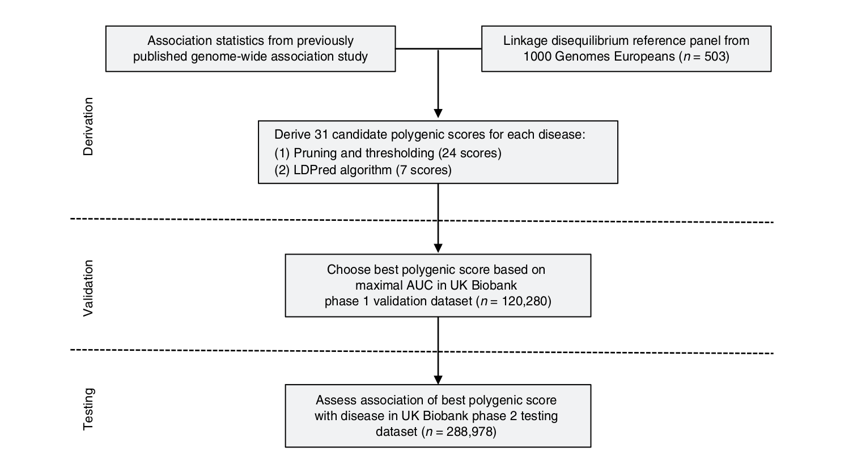
\includegraphics[width = 0.8 \textwidth]{figs/Imagen4.png}
\end{figure}

\newpage
Primero se cogieron estudios de GWAS que asocien el genotipo con un trait/enfermedad. Un panel de individuos permite calcular los bloques LD. Así, se crean 31 polygenic scores para cada enfermedad, 24 para el P+T y 7 para LDPred. Con la cohorte de Biobank se valida y se prueba en otra subcohorte. 

\begin{figure}[htbp]
\centering
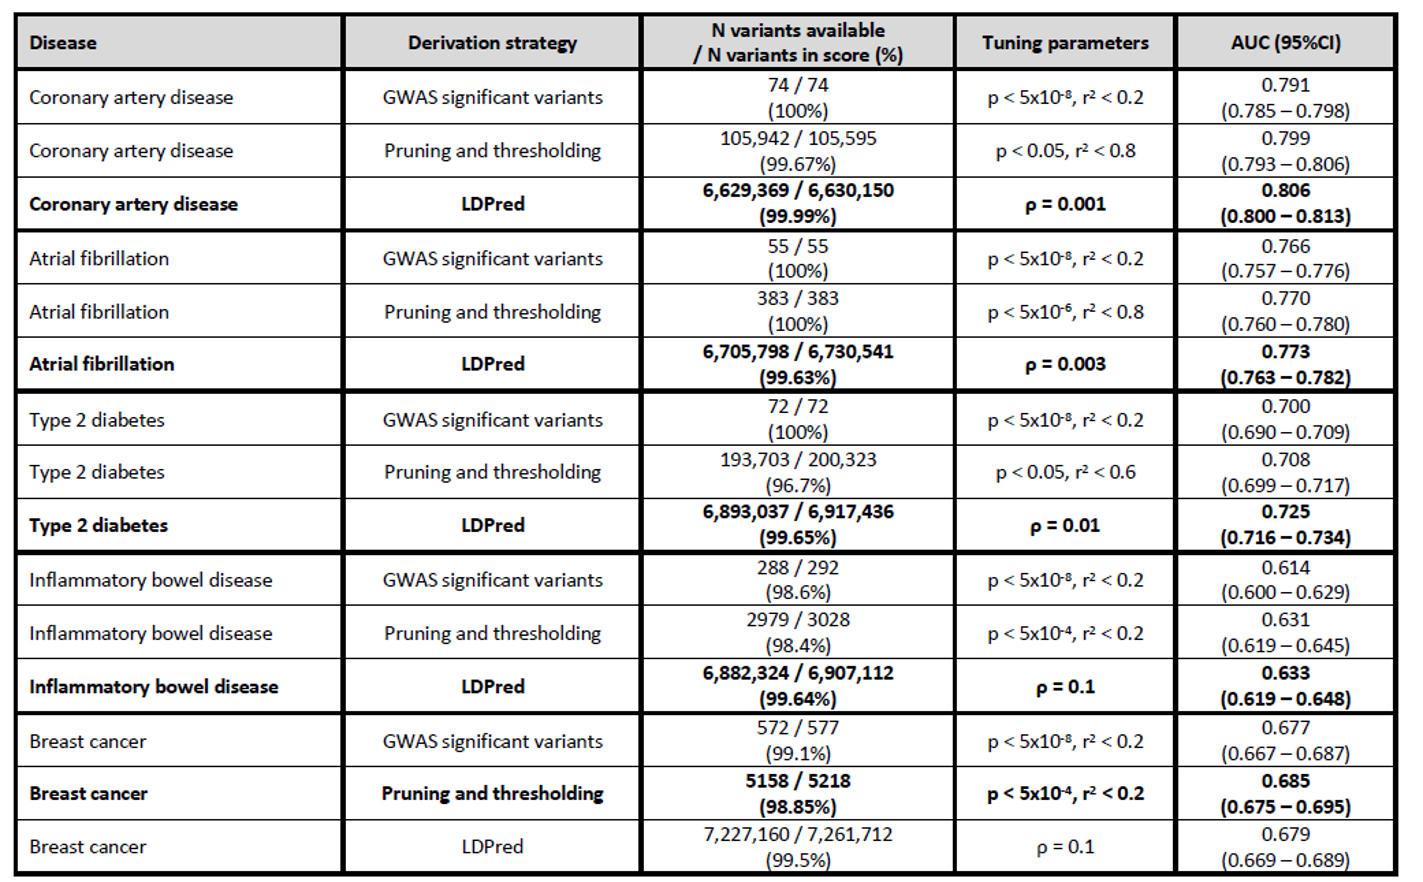
\includegraphics[width = 0.8 \textwidth]{figs/Imagen5.png}
\end{figure}

Para todas las enfermedades se calculó la predicción (el área bajo la curva) utilizando las variantes significativas en GWAS, la estrategia P+T y el algoritmo LDPred. Este método intenta repartir el efecto o la imagen duplicada/triplicada de los SNPs que se encuentran en el mismo LD, y se compara el dataset de validación y en el dataset de prueba. El área bajo la curva de ambos datasets son similares, lo que significa que los modelos funcionan bien para las poblaciones estudiadas.

\begin{figure}[htbp]
\centering
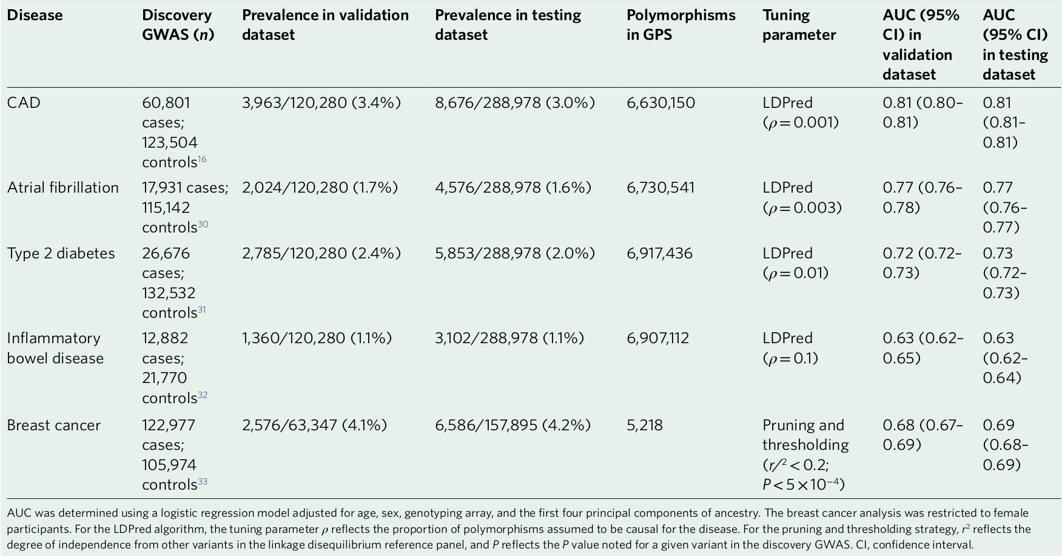
\includegraphics[width = 0.8 \textwidth]{figs/Imagen6.png}
\end{figure}

\newpage
En cuanto al riesgo de CAD acorde al GPS, se normalizó la distribución y se clasificó según el incremento del riesgo. El 8\% de la población tiene un riesgo 3x, el 2,3\% un riesgo 4x y un 0,5\% de la población un riesgo del 5x. El boxplot muestra que los casos tienen un mayor riesgo, y los controles un score menor.

\begin{figure}[htbp]
\centering
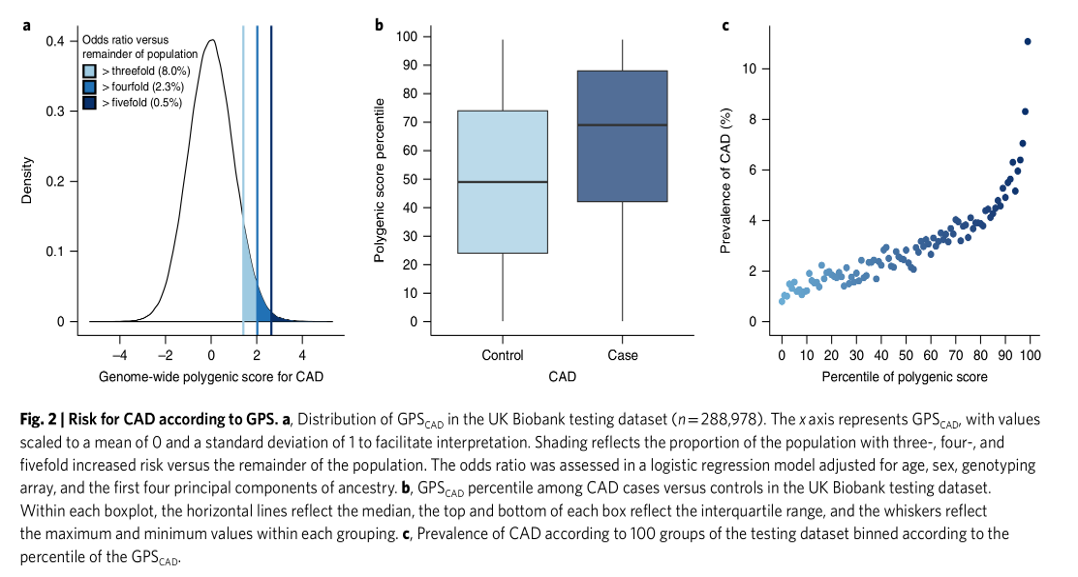
\includegraphics[width = \textwidth]{figs/Imagen7.png}
\end{figure}

\begin{figure}[htbp]
\centering
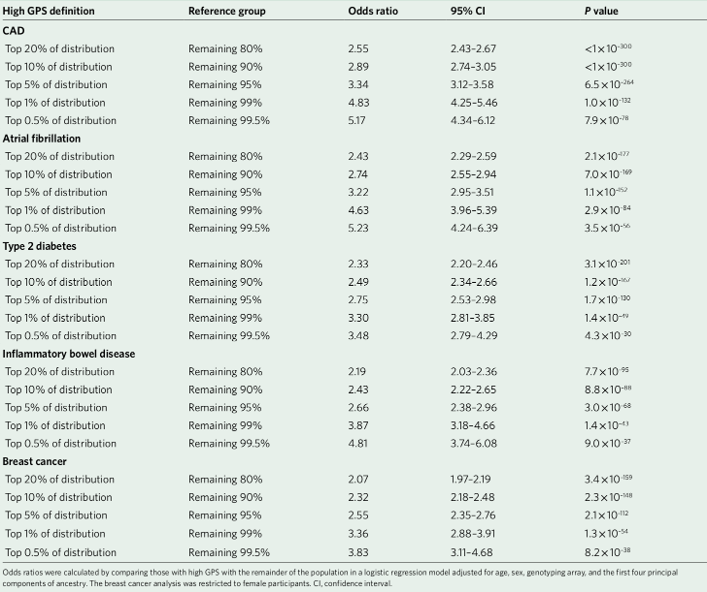
\includegraphics[width = 0.8 \textwidth]{figs/Imagen8.png}
\end{figure}

\newpage
En CAD hay un predictor para individuos con 3 veces más riesgo, que representan un 8\% de la población. También se muestran otros factores de riesgo y su nivel de significancia. Por ejemplo, fumar e hipertensión son factores de riesgo con un p-valor significativo. 
En la comparación entre individuos con un GPS alto y aquellos con puntajes promedio, las personas con un GPS alto tienden a tener otros factores de riesgo (por ejemplo, antecedentes familiares o niveles elevados de biomarcadores). Esto refuerza la utilidad del GPS como complemento a otras medidas de riesgo tradicionales.

\begin{figure}[htbp]
\centering
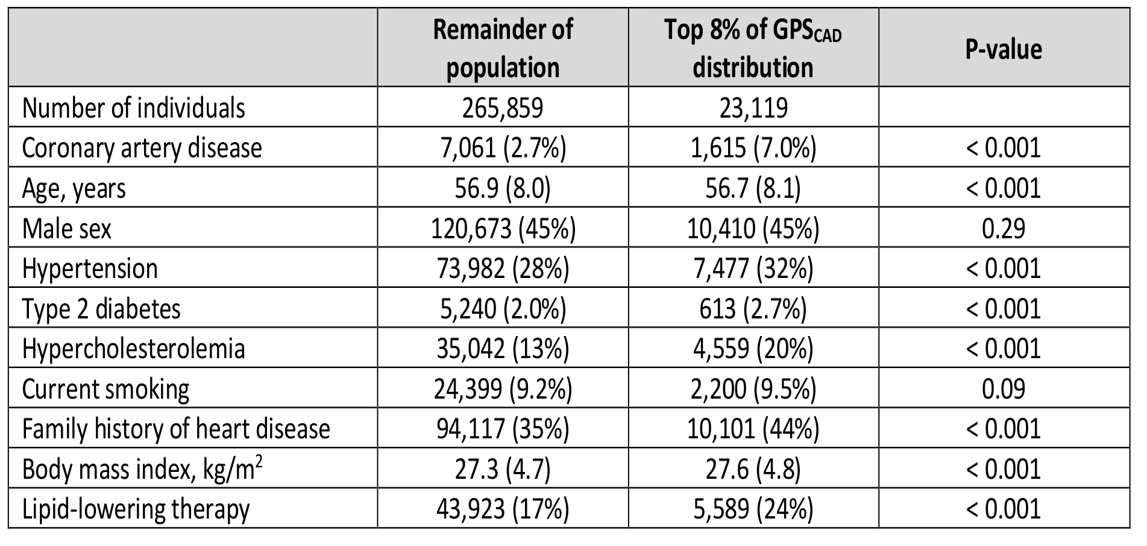
\includegraphics[width = 0.8 \textwidth]{figs/Imagen9.png}
\end{figure}

En conclusión:
\begin{itemize}
\item La posibilidad de identificar a los individuos con un riesgo genético significativamente mayor, en una amplia gama de enfermedades comunes y a cualquier edad, plantea una serie de oportunidades y retos para la medicina clínica.
\item Cuando se disponga de estrategias eficaces de prevención o detección precoz, las cuestiones clave serán la asignación de atención y recursos a individuos con distintos niveles de riesgo genético y la integración de la estratificación del riesgo genético con otros factores de riesgo, incluidas las mutaciones monogénicas raras y los factores clínicos y ambientales.
\item Cuando estas estrategias no existan o no sean óptimas, la identificación de los individuos de alto riesgo facilitará el diseño de estudios eficaces de la historia natural para descubrir marcadores precoces de la aparición de la enfermedad y de ensayos clínicos para probar estrategias de prevención.
\item El riesgo asociado a una puntuación poligénica elevada puede no reflejar un único mecanismo subyacente de patogenicidad. Prácticamente todas las enfermedades muestran un resultado final (la patología), pero lo que lleva a ella no se muestra.
\item La utilidad de los conocimientos y los posibles perjuicios para el individuo pueden variar en función de la enfermedad y la etapa de la vida. Será importante considerar cómo evaluar los riesgos absolutos y relativos y cómo comunicar estos riesgos para atender mejor a cada paciente; por ejemplo, para fomentar la adopción de modificaciones en el estilo de vida o el cribado de la enfermedad.
\item Las puntuaciones de riesgo poligénico aquí descritas se derivaron y probaron en individuos de ascendencia principalmente europea, por lo que no tendrán un poder predictivo óptimo para otros grupos étnicos.
\end{itemize}

%13/12 - Jorge de la Barrera
\chapter{Inherited Family Diseases}
\section{Conceptos genéticos clave}
Las enfermedades hereditarias tienen agregación familiar. 
A medida que se van produciendo generaciones de meiosis, los individuos van obteniendo segmentos más pequeños debido a la recombinación (distancia genética). Cuando se va haciendo recombinación homóloga, la distancia de las recombinaciones es la distancia genética.   
Un morgan se define como la distancia genética entre dos loci con una media de un evento de cruce por generación. No sucede igual en todas las regiones del genoma (debido al linkage desequilibrium). A medida que pasan las generaciones, la distancia genética va aumentando: la primera generación tiene 1/2 morgan (50 cM segmentos), pero en la generación k 1/k morgan, es decir, 100/k cM segmentos.

Identity by descent son regiones del genoma que se heredan de un mismo progenitor. Identity by state son regiones iguales, pero que no descienden del mismo antepasado; un genoma lo pudo heredar y el otro adquirir.

El desequilibrio de ligamiento (LD) se refiere a la asociación no aleatoria de alelos en dos o más loci genéticos. Los grupos de alelos permanecen heredados juntos como una unidad a lo largo de muchas generaciones, formando lo que se denominan bloques de LD. Las zonas que se recombinan más son más variables. Por regla general, si algo está muy conservado es porque es útil.

El SNP3 es el SNP causal, y el SNP que se caracteriza es el SNP4. En la población islandesa se verían lincados, pero en la francesa no. Estos bloques varían entre poblaciones. Siempre que se utilicen marcadores para marcar regiones del genoma y se vincula con ciertos traits, se puede dar este problema. 

\begin{figure}[htbp]
\centering
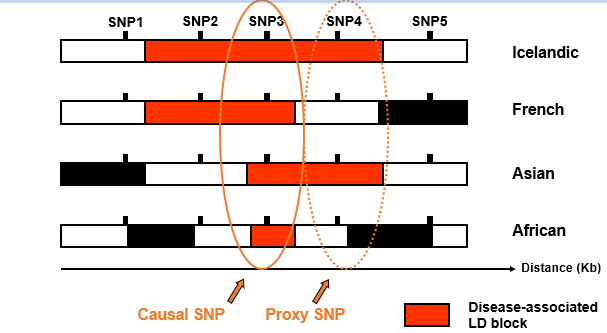
\includegraphics[width = 0.8\textwidth]{figs/ld-blocks.png}
\end{figure}

Cuando se genotipa, se pueden utilizar CHIPs o arrays. Sin embargo, actualmente se emplea más la secuenciación debido a su mayor capacidad para detectar variantes genéticas. En ambos casos, se obtiene el genotipo, pero no se puede determinar directamente si dos SNPs pertenecen al mismo cromosoma (materno/paterno) o están en cromosomas diferentes. Esta distinción es crucial. Por ejemplo, si un individuo tiene dos copias de un gen y ambas contienen mutaciones muy deletéreas, las consecuencias dependerán de cómo estén distribuidas:
Si ambas mutaciones están en una misma copia del cromosoma, la otra copia funcional puede compensar el defecto.
Si las mutaciones están repartidas en las dos copias (una en cada cromosoma), el individuo podría desarrollar la enfermedad.
La tarea de ordenar los genotipos según los cromosomas a los que pertenecen se denomina \textbf{phasing}.

\begin{figure}[htbp]
\centering
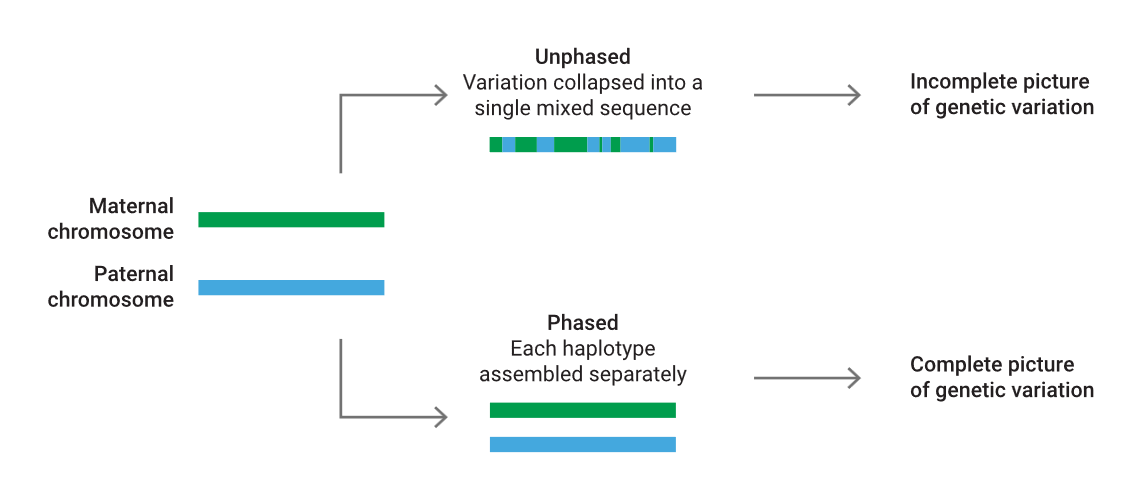
\includegraphics[width = \textwidth]{figs/Imagen1.png}
\end{figure}

Hay distintas formas de phasing:
\begin{itemize}
\item \textbf{Phasing físico:} Este método utiliza las lecturas físicas del genoma para inferir la fase. Las lecturas largas o tecnologías específicas como PacBio o Hi-C pueden ayudar a determinar directamente qué variantes están en el mismo cromosoma.

\item \textbf{Phasing por imputación (estadístico):} sabiendo las frecuencias de los alelos, se pueden inferir diferentes frecuencias en los datos. Esta misma idea se puede utilizar para inferir los haplotipos. La imputación suele capturar variantes frecuentes (polimorfismos). Para hacer el phasing estadístico, siempre es necesaria una referencia de haplotipos. Infiere la disposición de los alelos en cada uno de los cromosomas de un individuo (haplotipos) a partir de datos de genotipo que no especifican qué alelo está en cada cromosoma. Para ello, utiliza patrones de desequilibrio de ligamiento a nivel poblacional y haplotipos de referencia para resolver la fase incierta. Algoritmos como SHAPEIT, EAGLE y BEAGLE aplican modelos ocultos de Markov y paneles de referencia para mejorar la precisión del desfase. La precisión del desfase es esencial para identificar variantes causales en estudios de asociación de enfermedades, detectar segmentos de identidad por descendencia (IBD) y comprender los patrones de recombinación y la historia demográfica. Transforma los datos brutos de genotipo en información detallada de haplotipos, lo que permite realizar análisis genéticos y evolutivos más refinados.
\end{itemize}

El \textbf{equilibrio de Hardy-Weinberg} es el equilibrio de los genotipos en función de los alelos. Se utiliza en GWAS porque una variante que no esté en equilibrio se trata de una mutación reciente (que todavía se está equilibrando) o sufre de genetic drift. También puede darse a non-random mating (poblaciones cerradas y muy endogámicas) o por selección natural (que un genotipo no se establezca por ser muy deletéreo).

Hay fundamentalmente dos modelos: aditivo y dominante. En el aditivo, es necesario tener todas las copias de un gen para expresar un fenotipo, ya que se van sumando los efectos. En el modelo dominante, con tener una sola copia es suficiente para mostrar el fenotipo.

La \textbf{heredabilidad} se define como la proporción de la varianza fenotípica de un rasgo atribuible a factores genéticos. Tiene dos versiones:
\begin{itemize}
\item \textbf{Heredabilidad en sentido amplio ($H^2$):} Representa la proporción de varianza fenotípica explicada por todos los factores genéticos, incluidos los efectos aditivos, los efectos dominantes y los efectos epistáticos.

\item \textbf{Herencia en sentido estricto ($h^2$):} Mide específicamente la proporción de varianza fenotípica explicada por efectos genéticos aditivos, representando el grado en que los genes transmitidos por los padres determinan el fenotipo de su descendencia.
\end{itemize}

Varía entre 0,0 (ausencia de heredabilidad) y 1,0 (fuerte heredabilidad), y una puntuación a partir de 0,7 o 0,8 se considera que tiene una influencia grande en la heredabilidad de un rasgo.

$h^2$ se ha estimado tradicionalmente utilizando gemelos o familias. No obstante, ahora existen muchos métodos que permiten estimar la heredabilidad.

La \textbf{penetrancia} se refiere a la proporción de individuos portadores de una mutación específica que realmente presentan el fenotipo asociado. La \textbf{expresividad} describe la variación en la expresión fenotípica entre individuos portadores de la misma mutación.

La heterogeneidad genética se puede clasificar en dos tipos. La heterogeneidad del locus hace referencia a que las mutaciones en diferentes genes pueden provocar independientemente el mismo trastorno. En la heterogeneidad alélica, 
diferentes mutaciones dentro del mismo gen pueden producir la misma enfermedad.
\begin{figure}[htbp]
\centering
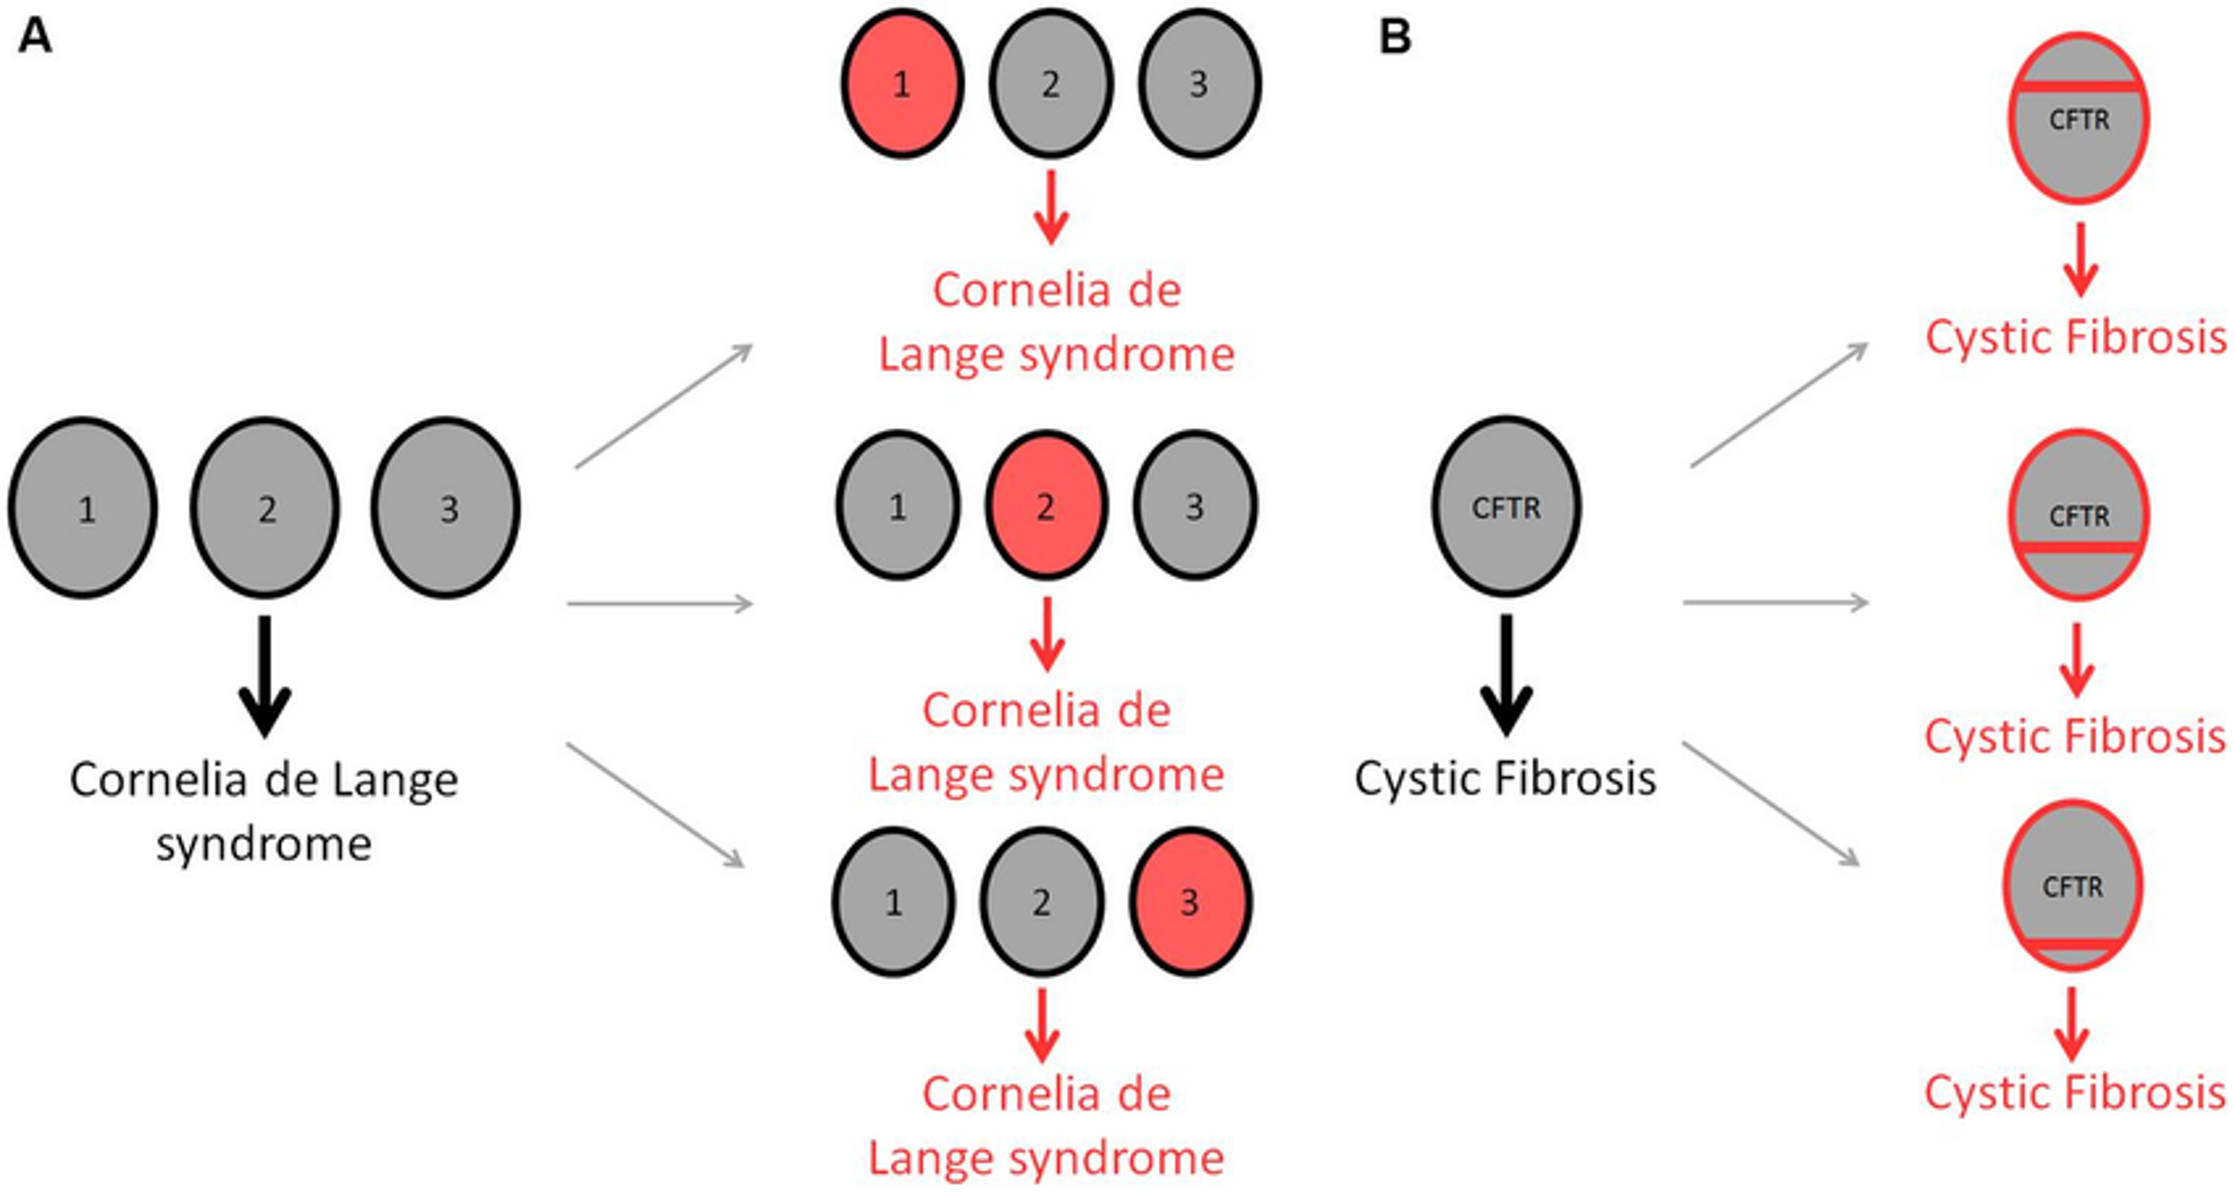
\includegraphics[width = \textwidth]{figs/genetic-heterogeneity.png}
\end{figure}

\section{Variantes genéticas en humanos}
El genoma humano tiene alrededor de 3,2 billones de pares de bases, o 3,2 Gb. Como somos diploides, en total son 6,4. La tasa de mutación es de $0,5 \cdot 10^{-8}$ a $1,5 \cdot 10{-8}$ por par de bases por generación. Así, salen unas 60-100 mutaciones de novo por generación. Todas las variantes compatibles con la vida existen en la población, pero la mayoría son rarísimas.

Como existe agregación familiar, se puede analizar el pedigrí para ver la segregación mendeliana.

\subsection{Linkage analysis}
El linkage analysis se utiliza para identificar regiones del genoma que se heredan conjuntamente con el fenotipo de una enfermedad, especialmente en enfermedades familiares. Estudiando los patrones de herencia en las familias, los investigadores pueden acotar las regiones genómicas que probablemente contengan genes causantes de enfermedades. La identificación de los segmentos que son IBD entre los individuos afectados puede señalar las regiones del genoma que probablemente contengan mutaciones causantes de la enfermedad. Ejemplo clásico: El descubrimiento del gen de la enfermedad de Huntington en el cromosoma 4.

Ligamiento es la tendencia de los alelos de los loci próximos a transmitirse juntos como una unidad intacta (haplotipo). La fracción recombinante ($\Theta$) varía entre 0,0 y 0,5, siendo 0,0 genes estrechamente ligados, sin recombinación y 0,5 no ligados, recombinación independiente. La distancia del mapa en centimorgans representa la longitud genética sobre la que se producirá un cruce recombinante en el 1\% de las meiosis.

El análisis de ligamiento basado en LOD implica la comparación de probabilidades de observar el patrón de segregación de 2 loci bajo modelos específicos, incluyendo una hipótesis nula de ausencia de ligamiento (surtido independiente - los loci se recombinan como si estuvieran en cromosomas diferentes) y una hipótesis alternativas de ligamiento (difieren en el grado de entrecruzamiento, es decir, diferentes valores de eventos de recombinación).
$$Z = \frac{\text{Likelihood of the data if loci linked at a particular} \Theta}{\text{Likelihood of the data if loci are unlinked} (\Theta = 0.5)}$$

\begin{figure}[htbp]
\centering
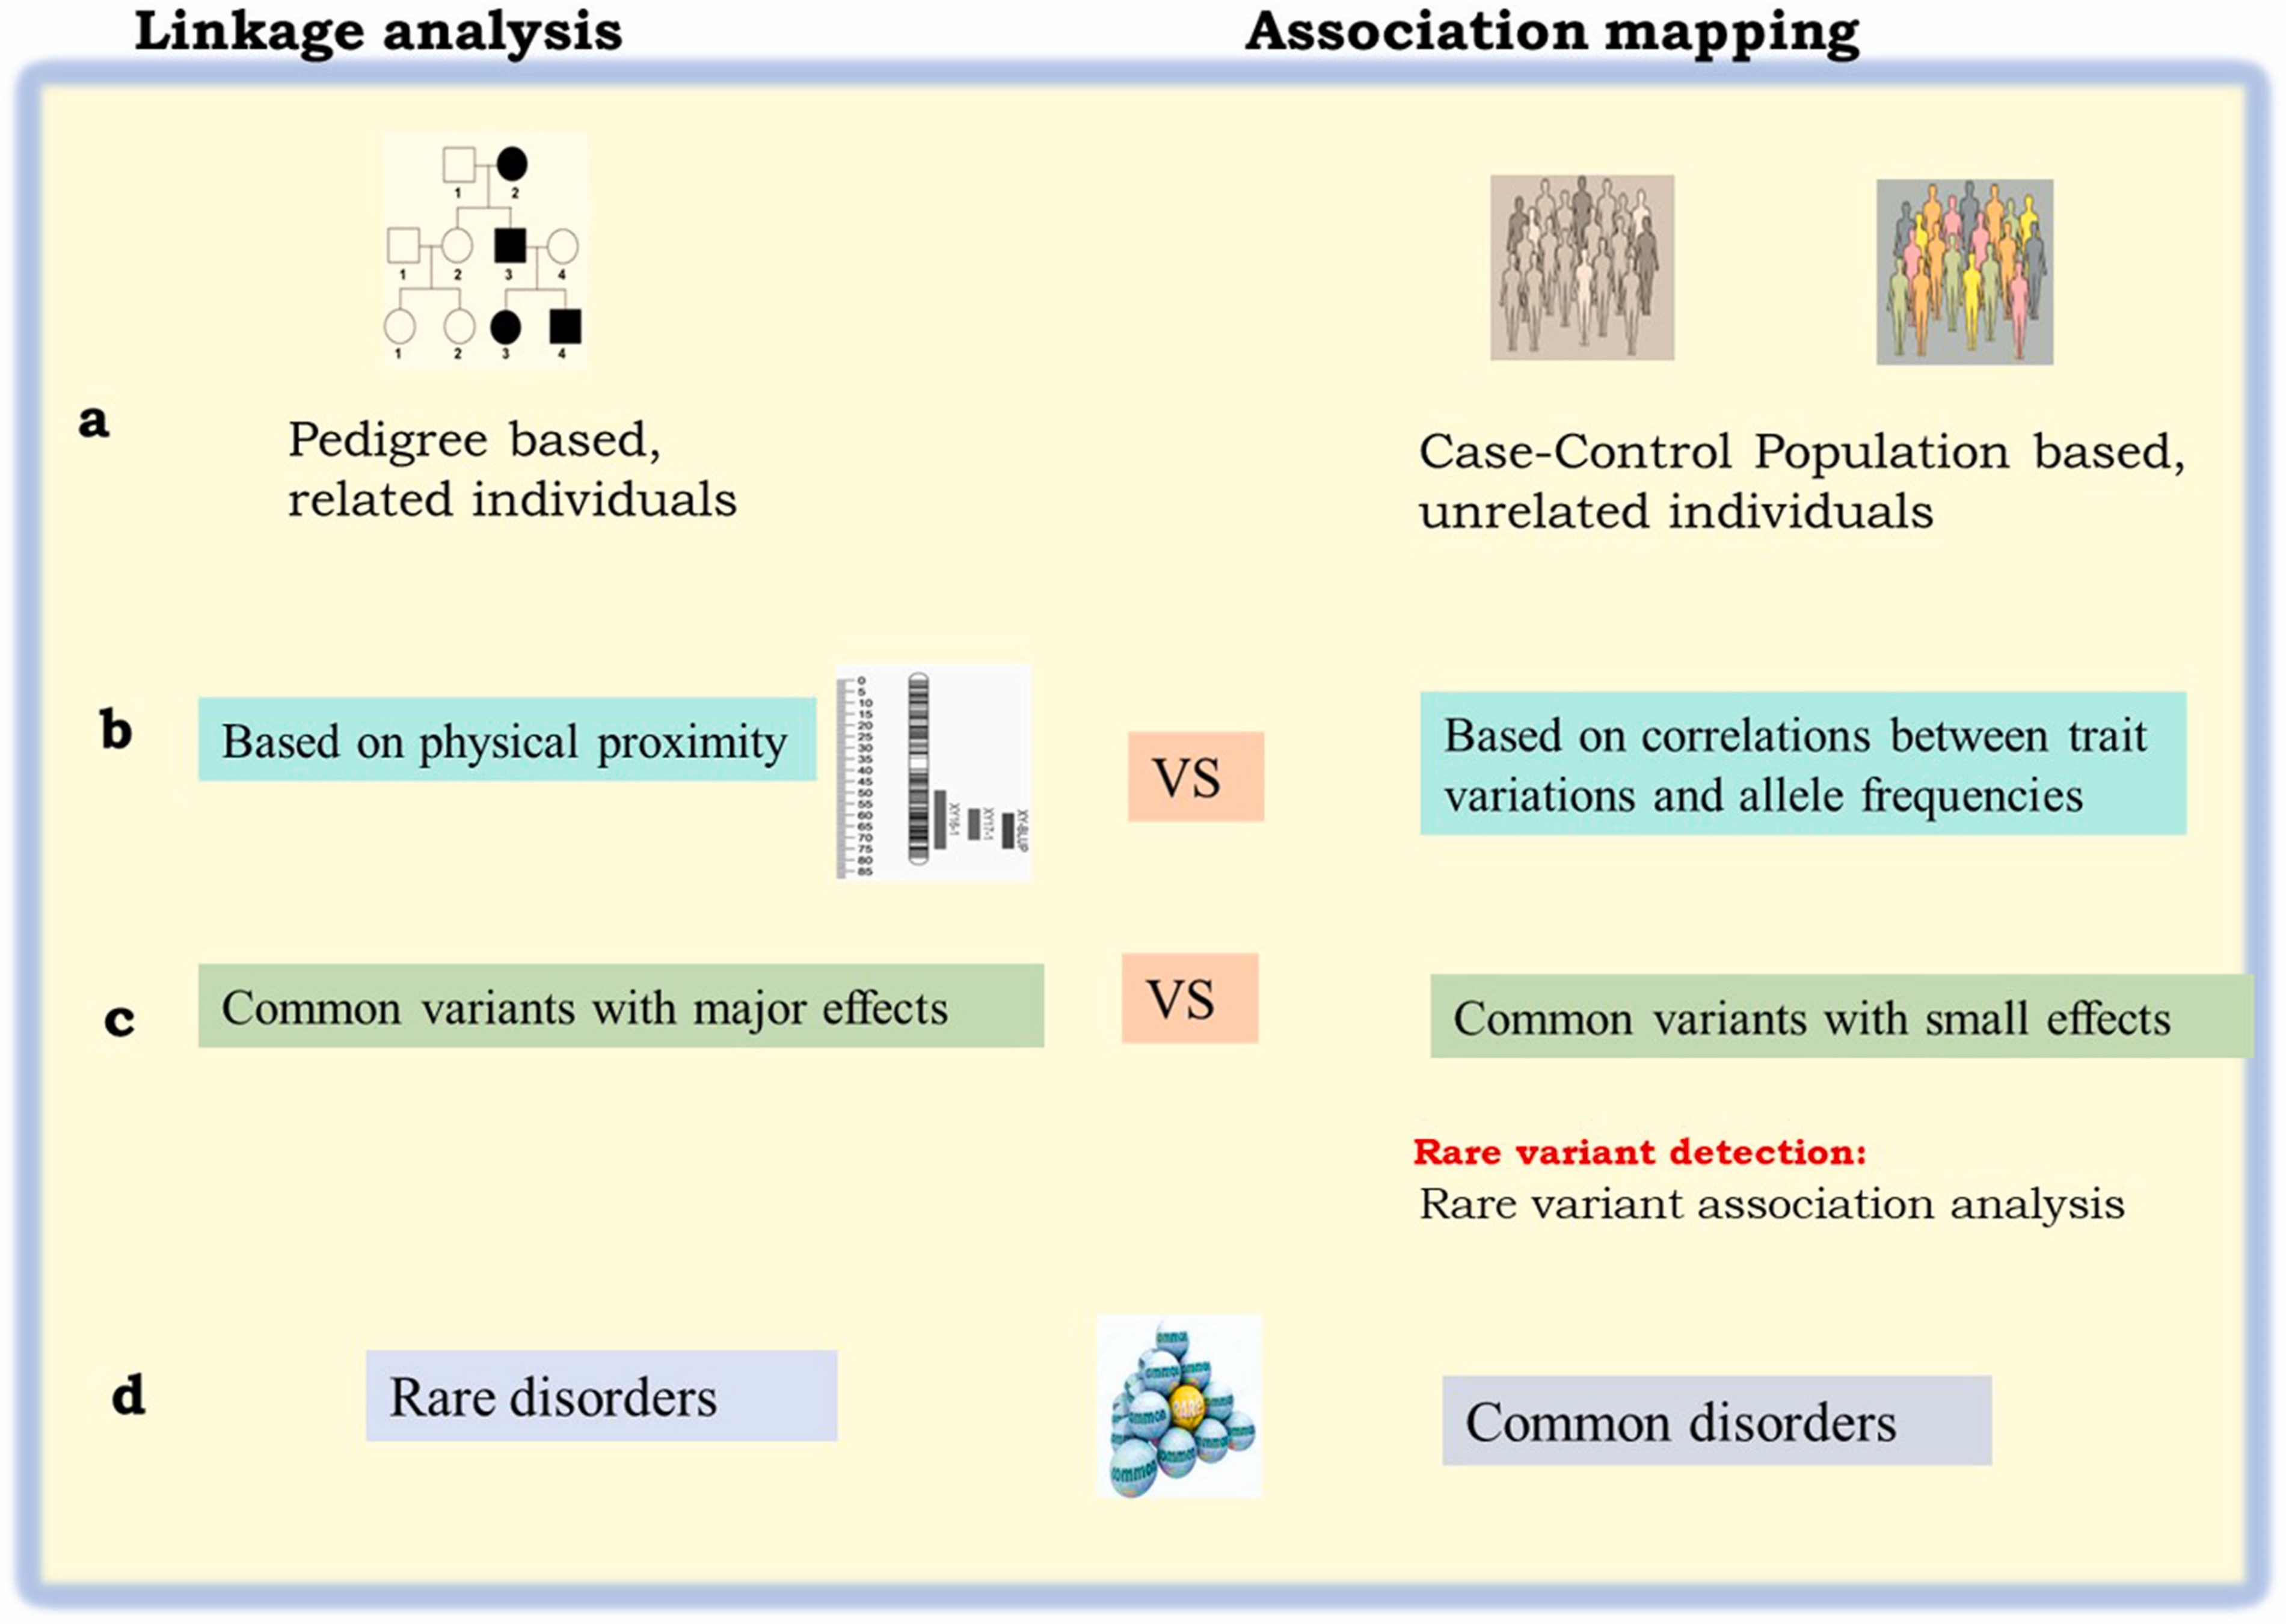
\includegraphics[width = 0.8\textwidth]{figs/Imagen3.jpg}
\end{figure}

\subsection{Family-based analysis}
En el análisis por familias, se utilizan los datos de individuos estrechamente emparentados -como padres, hijos y hermanos- para investigar la base genética de rasgos o enfermedades.

\begin{figure}[htbp]
\centering
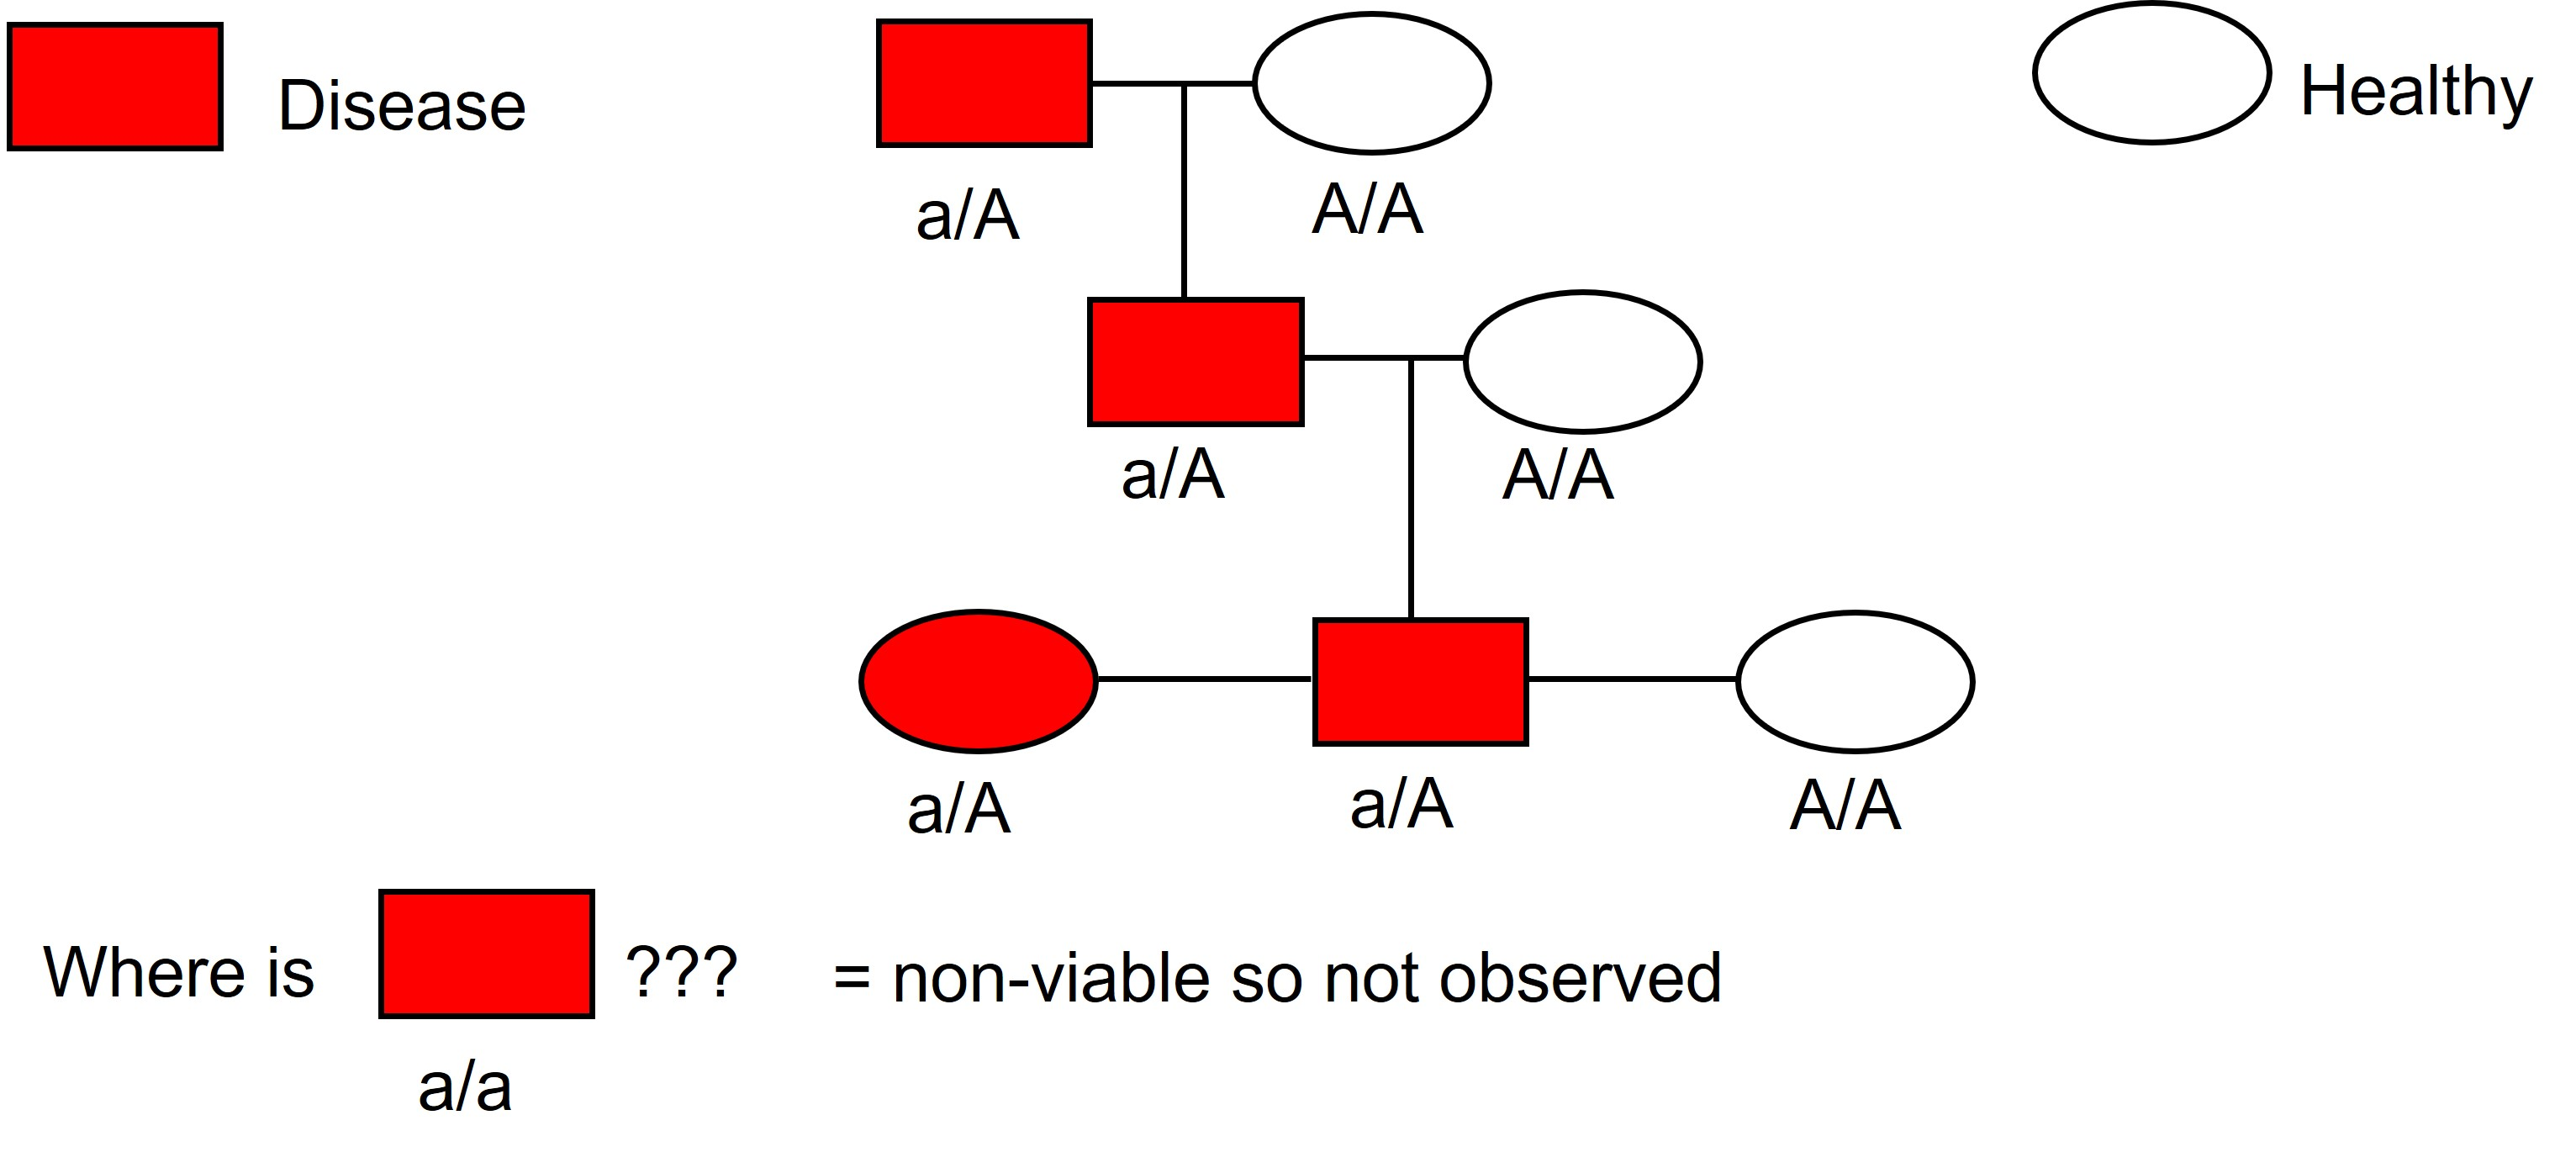
\includegraphics[width =0.8 \textwidth]{figs/Imagen4.jpg}
\end{figure}

En este ejemplo, no se ve ningún genotipo con los dos alelos menores. Se utiliza el supuesto de que no se observa al no ser viable (deletéreo). 

La \textbf{prueba de desequilibrio de transmisión (TDT)} comprueba si un alelo en un locus determinado (relacionado con una enfermedad o rasgo) es transmitido a la descendencia afectada por los progenitores con más frecuencia de lo esperado por azar. Los padres heterocigotos transmiten los alelos m1 y m2 en un locus determinado con la misma frecuencia (50\%); la descendencia afectada debería recibir el alelo asociado a la enfermedad con mayor frecuencia. No es necesario un grupo de control, y es resistente a la estratificación de la población en el análisis de asociación basado en la familia.

\begin{figure}[htbp]
\centering
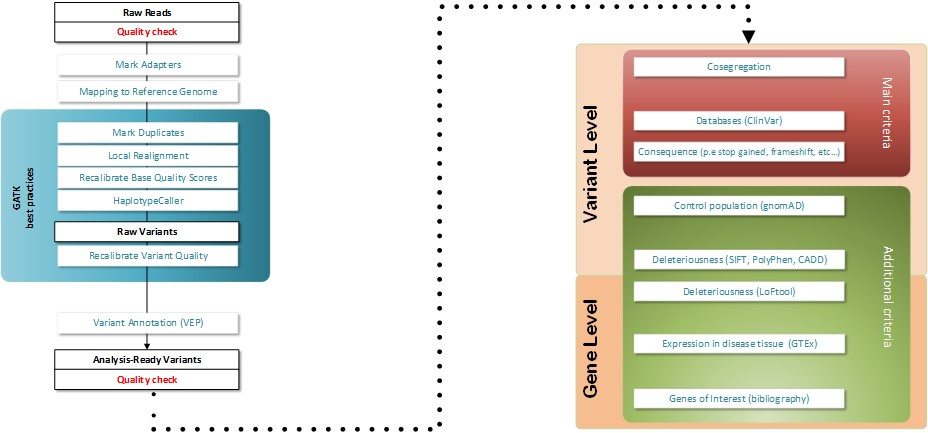
\includegraphics[width = \textwidth]{figs/Imagen5.jpg}
\end{figure}

\begin{figure}[htbp]
\centering
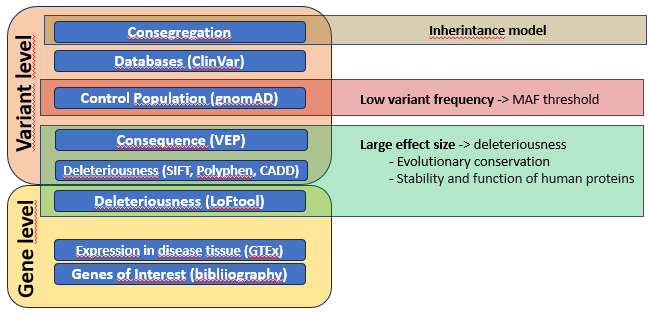
\includegraphics[width = 0.8\textwidth]{figs/filtering_approaches.png}
\end{figure}

\begin{table}[htbp]
\centering
\begin{tabular}{p{3cm}|p{8cm}|p{4cm}}
Modelo de herencia & Características clave & Ejemplos de enfermedades \\ \hline
Autosómica dominante & Una copia del gen mutado es suficiente, afecta a ambos sexos & Enfermedad de Huntington, poliposis adenomatosa familiar \\
Autosómica recesiva & Se necesitan dos copias del gen mutado, portadores sanos & Fibrosis quística, anemia de células falciformes \\
Ligada al X (dominante) & Afecta a ambos sexos, mujeres menos afectadas, transmitida por hombres a todas sus hijas & Síndrome de Rett \\
Ligada al X (recesiva) & Afecta principalmente a hombres, mujeres son portadoras & Hemofilia \\
Ligada al Y & Solo afecta a hombres, transmitida de padres a hijos & Algunas formas de infertilidad masculina \\
Mitocondrial & Transmitida por la madre, afecta a ambos sexos & Neuropatía óptica hereditaria de Leber \\
Multifactorial & Influencia de múltiples genes y factores ambientales & Enfermedades cardíacas, diabetes tipo 2
\end{tabular}
\end{table}

Para variantes de baja frecuencia en la población, se establece un límite MAF compatible con la prevalencia de la enfermedad en la población: monogénica/variante única y oligogénica/variantes múltiples. Para medir el efecto, se utilizan distintos predictores:
\begin{itemize}
\item \textbf{SIFT (Sorts Intolerant from Tolerant):} funciona a nivel de variantes. Toma una secuencia de consulta y utiliza información de alineamiento múltiple para predecir sustituciones toleradas y deletéreas para cada posición de la secuencia de consulta. SIFT es un procedimiento de varios pasos que busca secuencias similares, elige secuencias estrechamente relacionadas que puedan compartir una función similar a la secuencia de consulta, obtiene la alineación de estas secuencias elegidas y calcula las probabilidades normalizadas de todas las posibles sustituciones a partir del alineamiento. Las posiciones con probabilidades normalizadas inferiores a 0,05 se consideran deletéreas, mientras que las superiores o iguales a 0,05 se consideran toleradas.
\item \textbf{PolyPhen (Polymorphism Phenotyping):} funciona a nivel de variantes. Predice el posible impacto de las sustituciones de aminoácidos en la estabilidad y función de las proteínas humanas utilizando consideraciones estructurales y evolutivas comparativas. Realiza una anotación funcional de polimorfismos de un solo nucleótido (SNP), asigna SNP codificantes a transcripciones de genes, extrae anotaciones de secuencias de proteínas y atributos estructurales y construye perfiles de conservación. Estima la probabilidad de que la mutación de sentido erróneo sea perjudicial basándose en una combinación de todas estas propiedades.
\item \textbf{CADD (Combined Annotation-Dependent Depletion):} funciona a nivel de variantes (incluidas las no codificantes). Prioriza variantes causales particularmente contribuyentes altamente penetrantes a desórdenes Mendelianos severos. Puede puntuar SNV humanas e INDELS cortas El entrenamiento del modelo CADD requiere la identificación de variantes que son fijas o casi fijas en poblaciones humanas, pero que están ausentes en la secuencia genómica inferida del ancestro humano-ape (variantes proxy-neutrales). La composición de la secuencia de este conjunto de variantes se utiliza para dibujar un conjunto coincidente de variantes proxy-deletéreas. Utilizando más de 60 anotaciones diversas, se entrena un modelo de aprendizaje automático para clasificar las variantes como proxy-neutrales frente a proxy-deletéreas. Todas las SNV potenciales del genoma humano de referencia se anotan utilizando las mismas características, y se calculan las puntuaciones crudas de CADD. Se obtiene una tabla de conversión PHRED a partir de la clasificación relativa de los núcleos de estos modelos.

\begin{figure}[htbp]
\centering
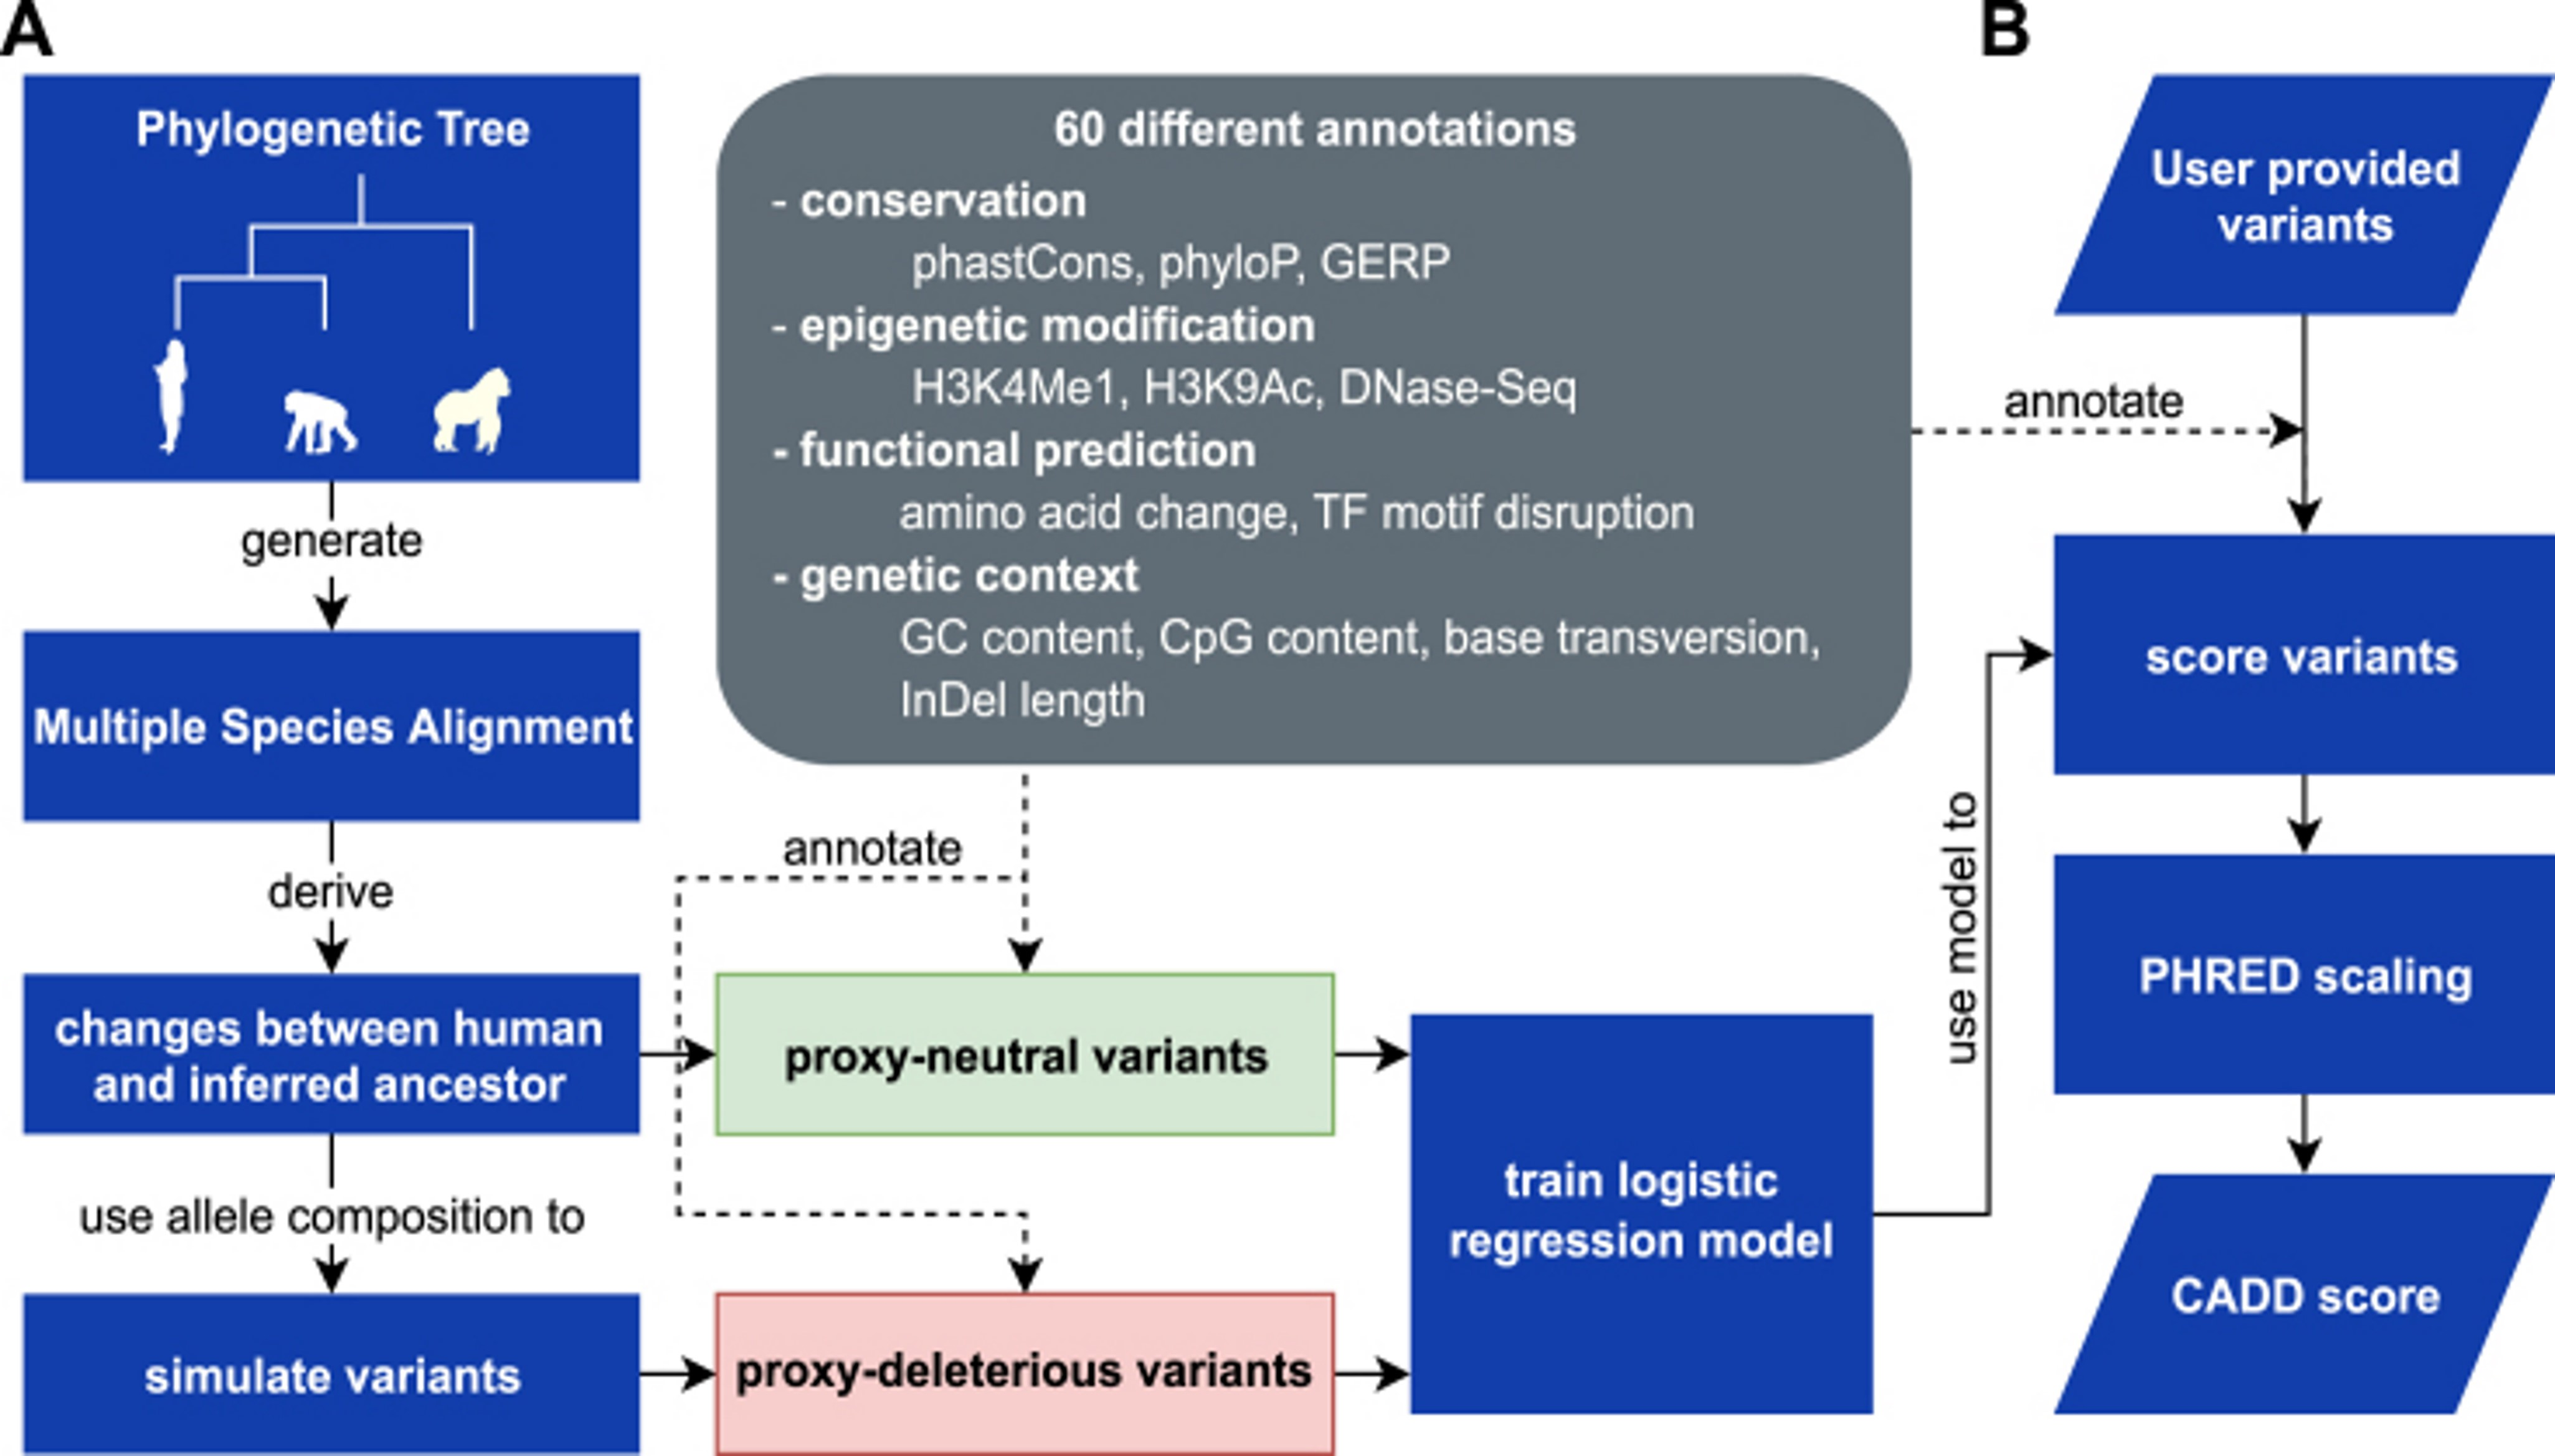
\includegraphics[width = 0.7\textwidth]{figs/cadd.jpg}
\end{figure}

\item \textbf{LoFtool (Depletion of loss-of-function):} LoF en 60 706 individuos no emparentados y muestran que el cuartil más intolerante de genes clasificados está enriquecido en enfermedades raras y de aparición temprana y explica el 87\% de las mutaciones OMIM haploinsuficientes de novo, un 17\% más que cualquier otra herramienta de puntuación de genes. Las mutaciones LoF de alta confianza se definieron aquí como variantes con ganancia de parada, alteración del sitio de empalme y desplazamiento de marco que no son el alelo ancestral (en todos los primates), en el último 5\% del transcrito, en exones e intrones con sitios de empalme no canónicos a su alrededor, en intrones de menos de 15 pb, en genes con un solo exón y en sitios aceptores rescatados por un sitio aceptor dentro del marco.
\end{itemize}

Otras fuentes externas pueden ser ClinVar (recoge datos sobre variantes genéticas y sus efectos asociados, tanto patógenos como benignos, en las enfermedades humanas), Genotype-Tissue Expression GTEx (ofrece una visión detallada de la expresión génica en los tejidos humanos y su relación con la variación genética) y bibliografía de los genes de interés. 

\section{Práctica: paper}
Para ver estos conceptos de forma práctica, analizaremos el papel "A Human Hereditary Cardiomyopathy Shares a Genetic Substrate With Bicuspid Aortic Valve". Se analizaron varias familias por la presencia y ausencia de R530X y V943F. Se trata de una enfermedad oligogénica que se hereda junta. 

\begin{figure}[htbp]
\centering
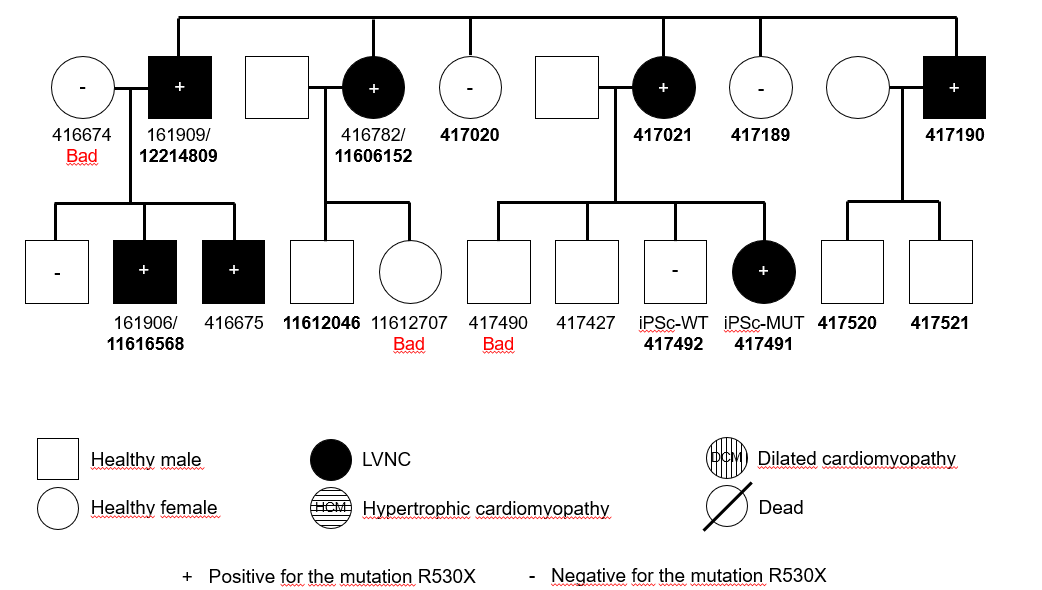
\includegraphics[width = \textwidth]{figs/pedigri1.png}
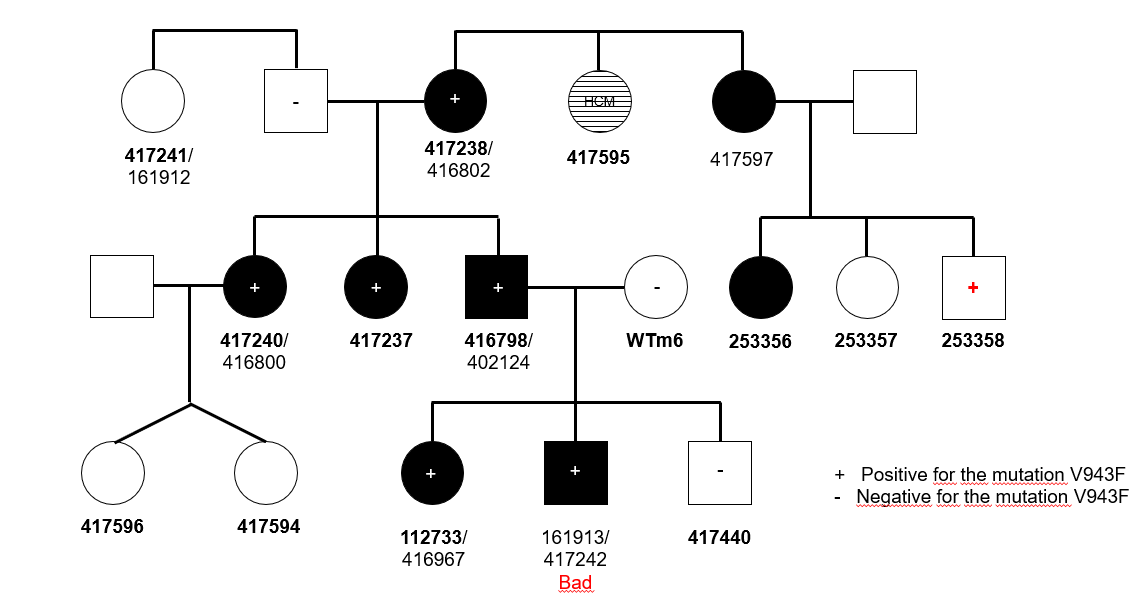
\includegraphics[width = \textwidth]{figs/pedigri2.png}
\end{figure}

\begin{figure}[htbp]
\centering
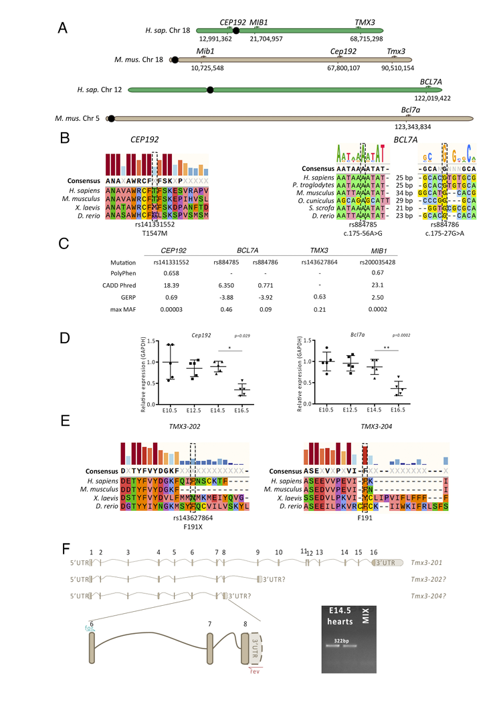
\includegraphics[width = 0.85\textwidth]{figs/Imagen1-paper.png}
\caption{(A) Localización cromosómica de los genes identificados en humanos y ratones. (B) Conservación de las secuencias de aminoácidos y ADN en las regiones afectadas en las variantes. (C) Principales predictores y datos de prevalencia de las variantes identificadas. (D) Análisis qPCR de los genes candidatos en corazones de ratón en diferentes estadios de desarrollo, en relación con la expresión de GAPDH. Ambos genes mostraron una expresión dinámica a lo largo del periodo examinado.  (E) La región C-terminal de la proteína codificada por la isoforma 202 de TMX3 no está conservada (panel izquierdo), pero la mutación introducida en el genoma del ratón afecta a una Phe conservada (panel derecho). (F) Estructura genética de la Tmx3 de ratón. El homólogo de ratón de la principal isoforma humana comparte su estructura, pero sólo existe un transcrito codificador de proteína en ratón. }
\end{figure}